\section{Introduction}

\begin{frame}
	\frametitle{Discretization and reconstruction of signals}
	\begin{definition}
	The use of digital logic and computers to calculate a control action for a continuous system introduces the operation of sampling. Samples are taken from the continuous signals and used in the computer to calculate the controls to be applied.\\
	\end{definition}
	\vspace{1em}
	\begin{columns}
		\begin{column}{0.5\textwidth}
			The role of sampling and the conversion from continuous to discrete and vice versa are important to the understanding of the complete response of digital control.
		\end{column}
		\begin{column}{0.5\textwidth}
			\vspace{-0.8em}
			\begin{figure}
			\centering
			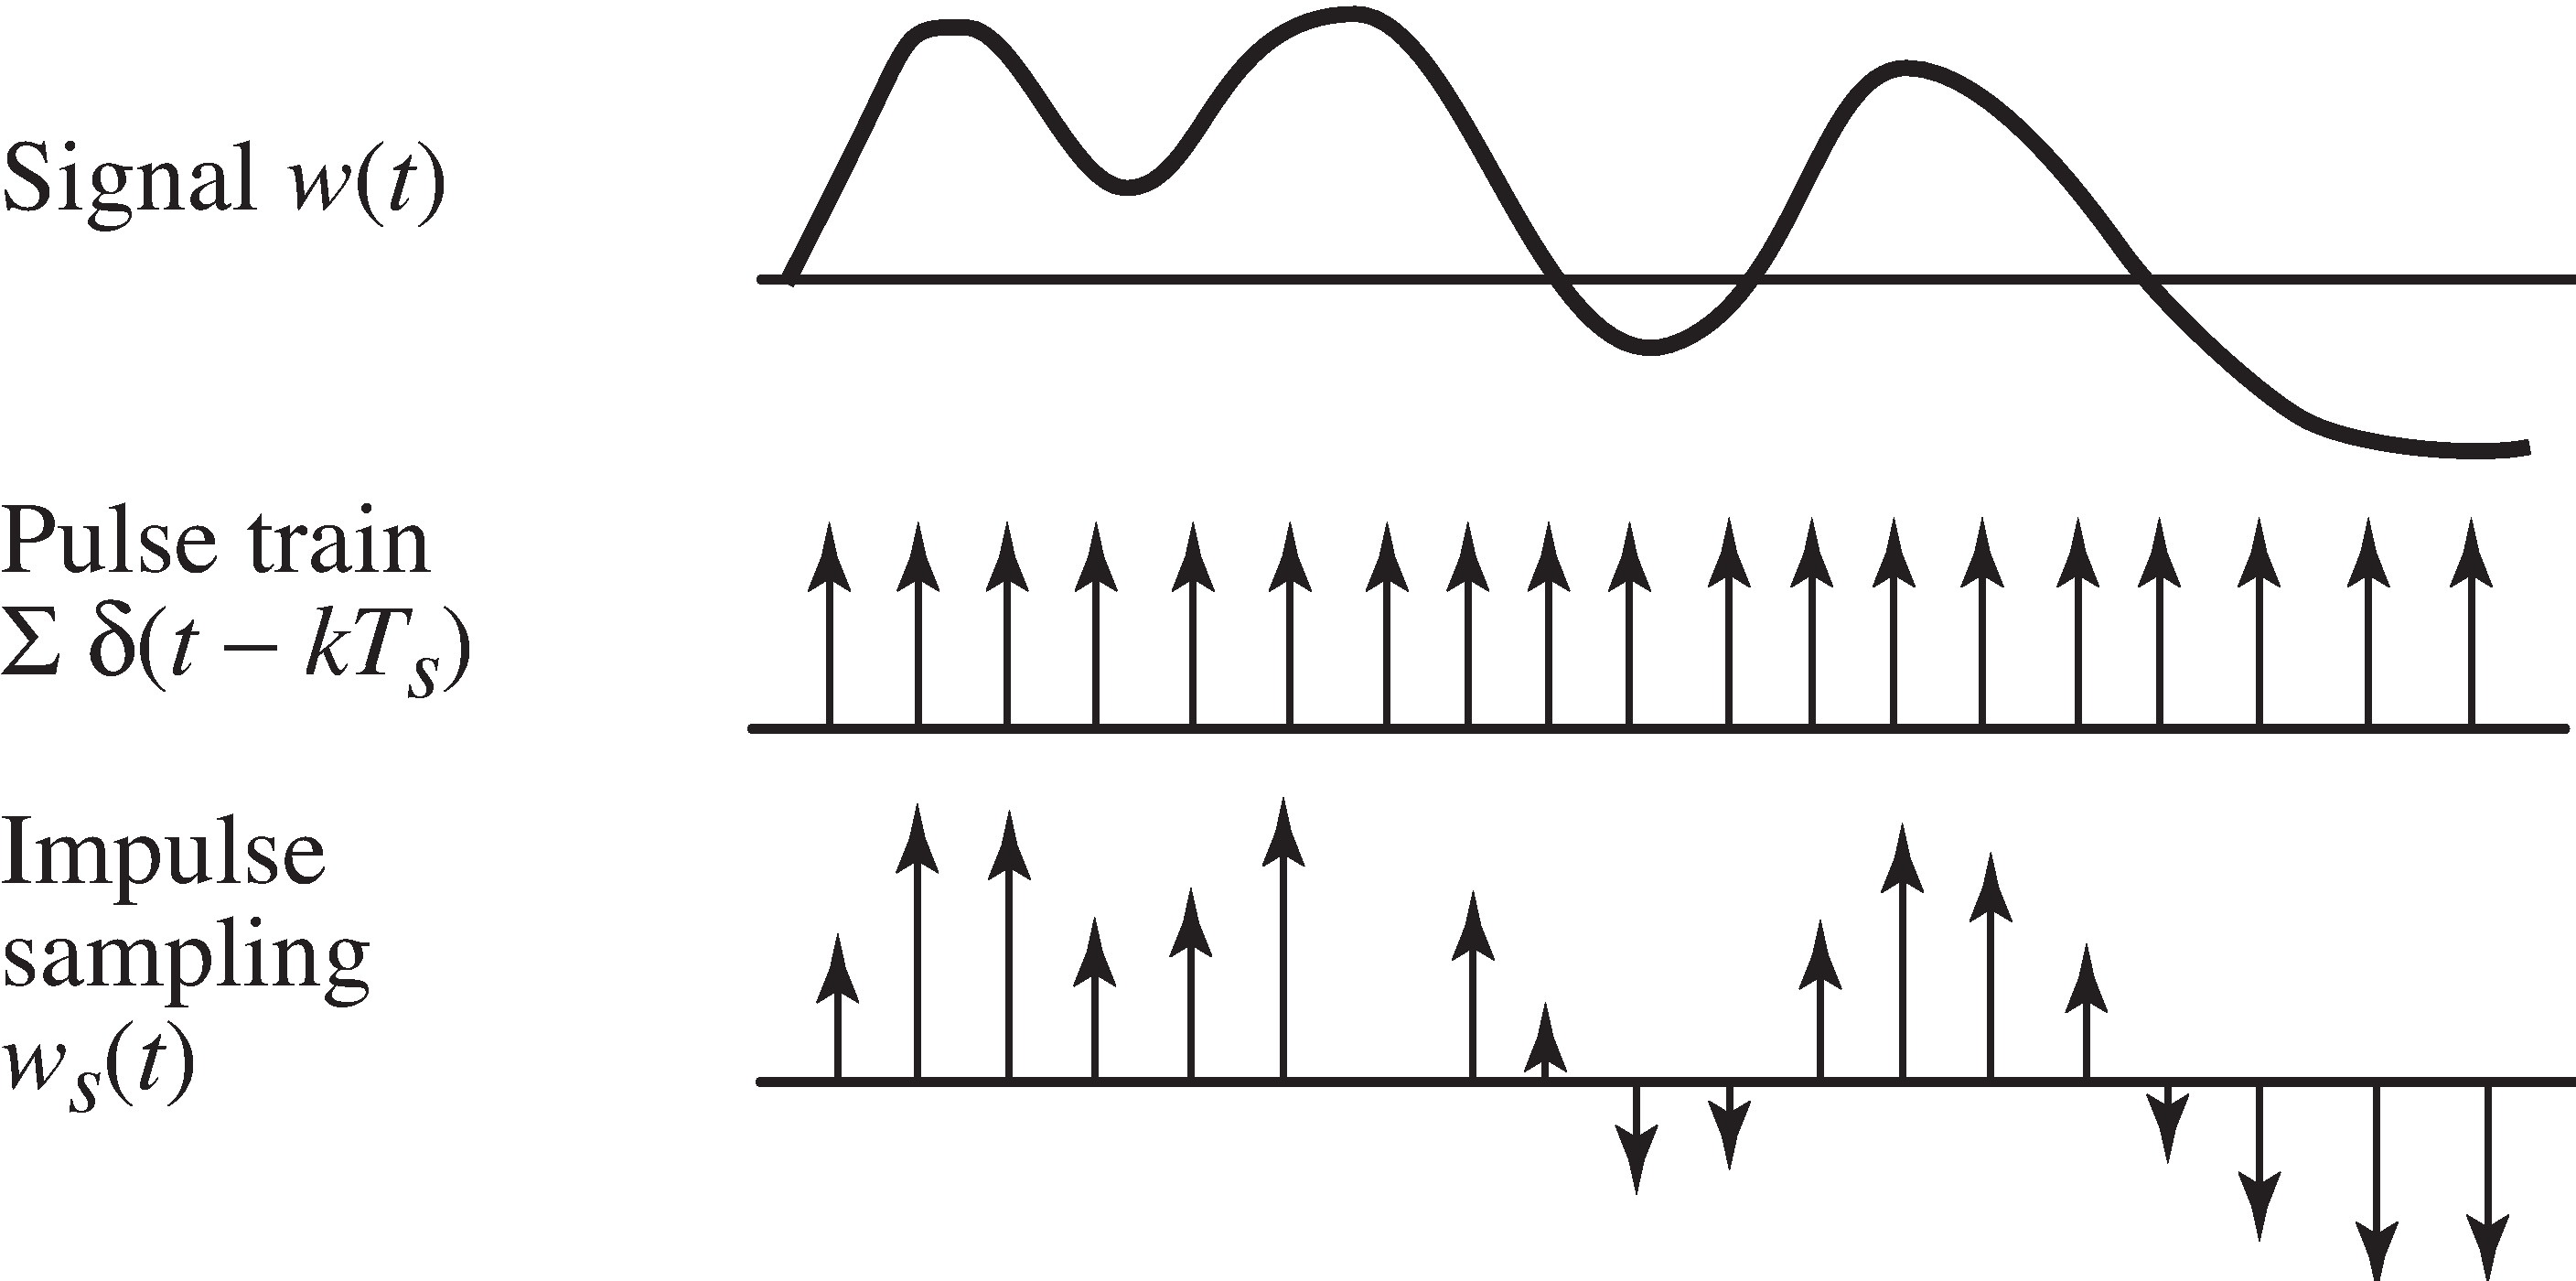
\includegraphics[width=1\linewidth]{discretization}
			\end{figure}
		\end{column}
	\end{columns}
	%source: http://cnx.org/contents/42c54126-3078-417f-972e-dcf5c41556a4@3.1:6/Software-Receiver-Design
\end{frame}

\begin{frame}
	\frametitle{Types of signals}
	\begin{itemize}
		\item \textbf{Continuous-time signal}: A signal defined over a continuous range of time.
		\item \textbf{Discrete-time signa}l: A signal defined only at discrete instants of time (the independent variable t is quantized)
		\item \textbf{Analog signal}: A signal defined over a continuous range of time whose amplitude can assume a continuous range of values.
		\item \textbf{Quantized signal}: A signal in which the amplitude may assume only a finite number of distinct values.
	\end{itemize}
\end{frame}

\begin{frame}
	\frametitle{Types of signals}
	\begin{columns}
		\column{0.6\textwidth}
		a. Continuous-time analog signal\\
		\medskip
		b. Continuous-time quantized signal\\
		\medskip
		c. Sampled-data signal (discrete-time analog signal)\\
		\medskip
		d. Digital signal (discrete-time quantized signal)
		\column{0.4\textwidth}
		\vspace{-2ex}
		\begin{figure}
			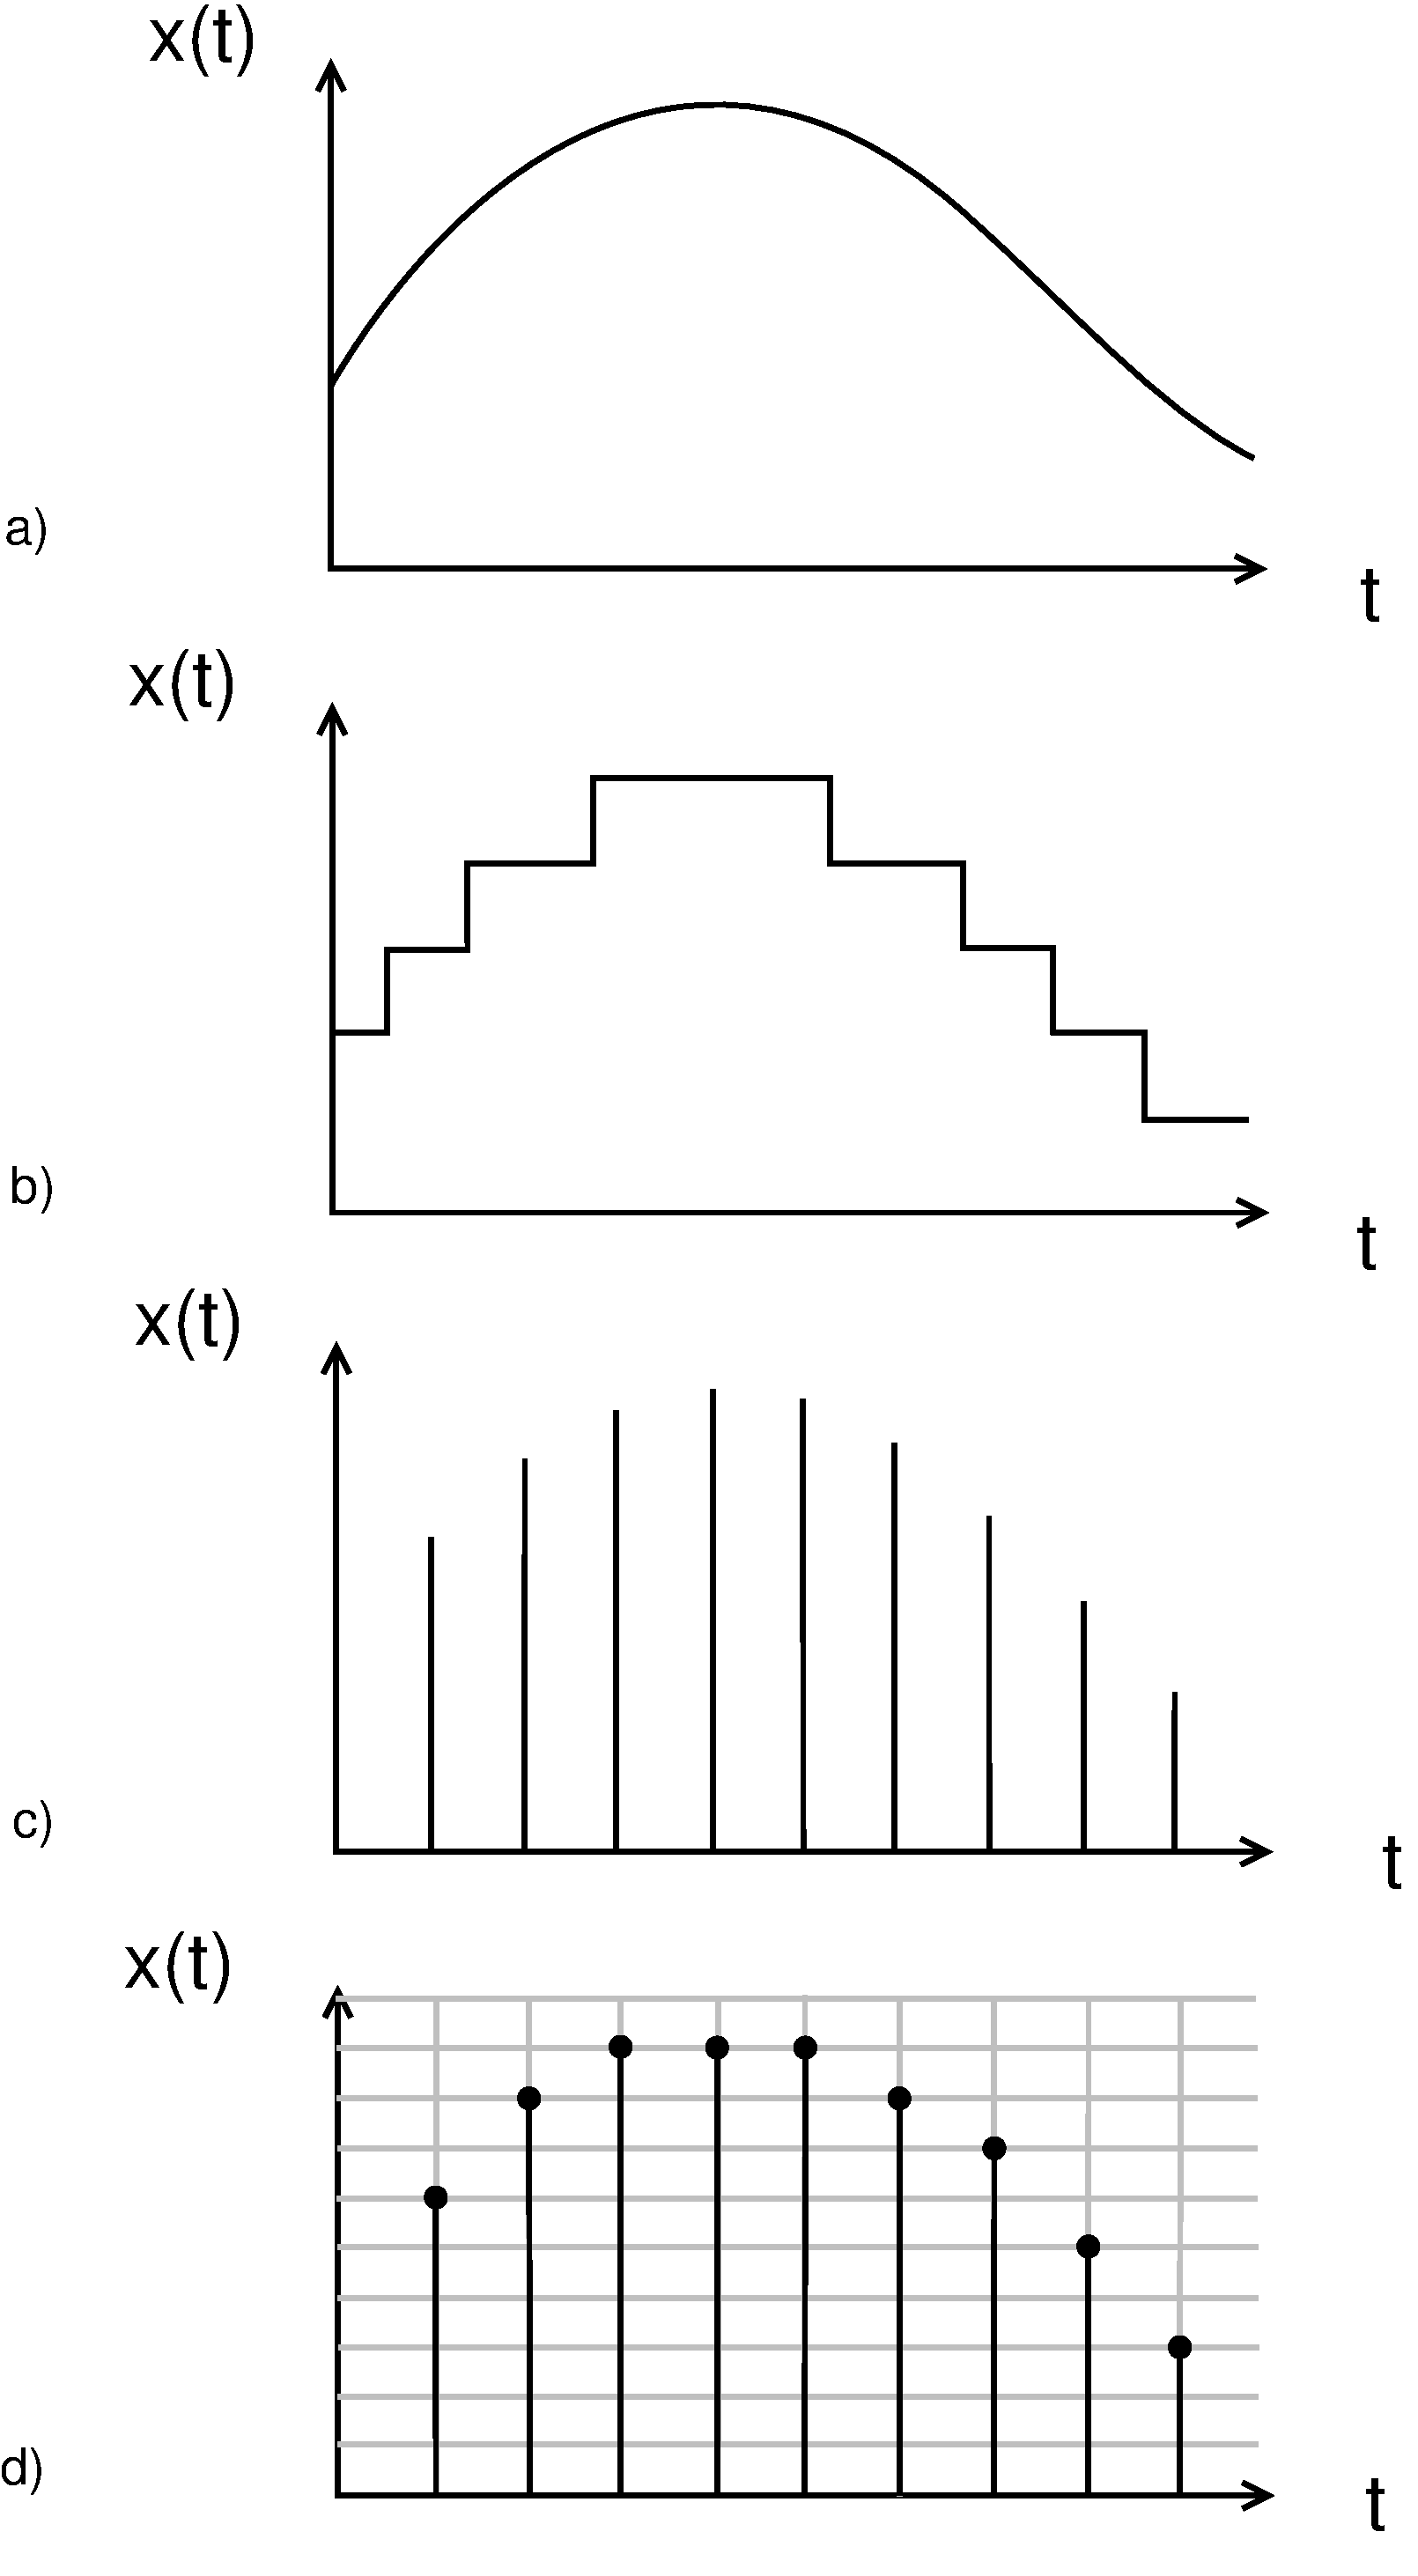
\includegraphics[width=0.8\linewidth]{types}
		\end{figure}
	\end{columns}
\end{frame}

\begin{frame}
	\frametitle{Digital control system}
	\begin{figure}
		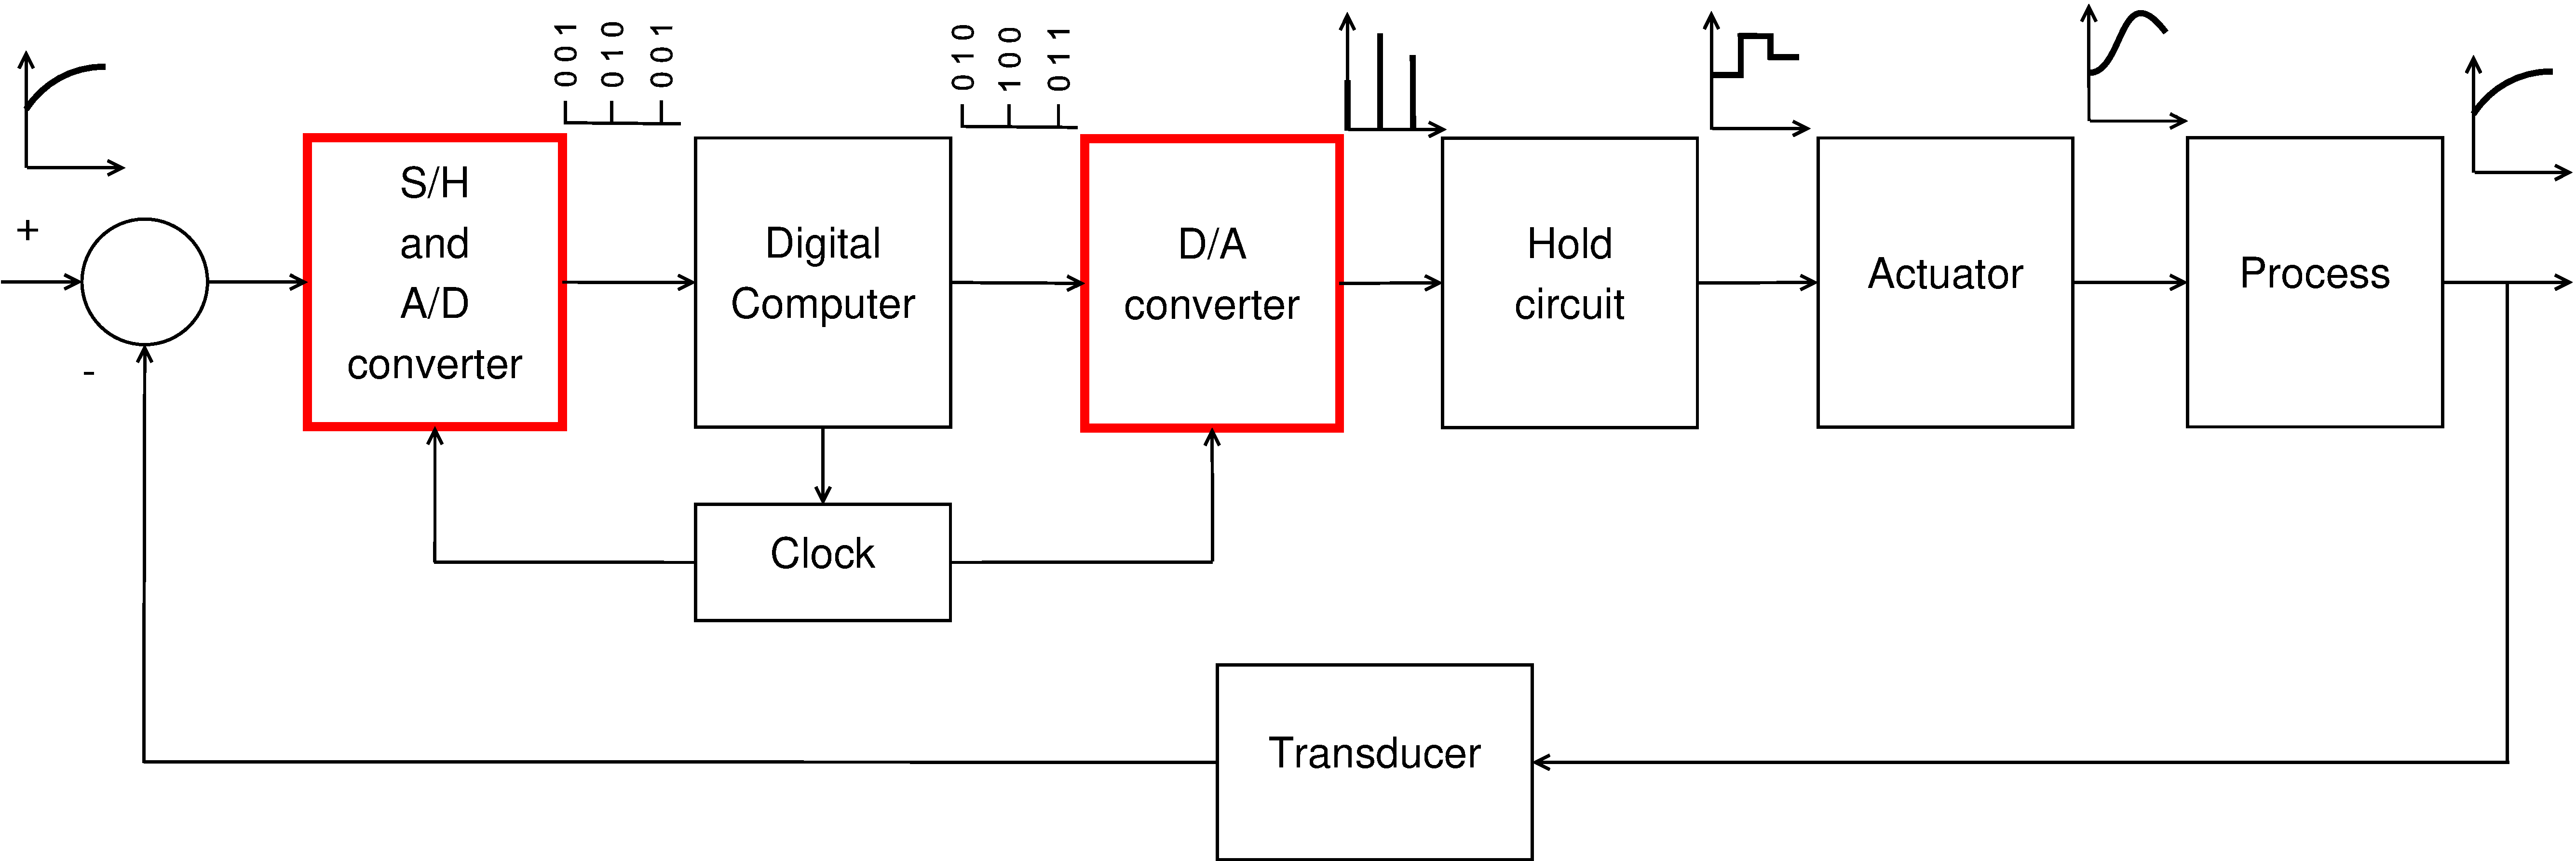
\includegraphics[width=1\textwidth]{digital_control_system}
	\end{figure}
\end{frame}

\begin{frame}
	\frametitle{Definitions}
	\begin{block}{}
	\textbf{Sample and hold}\\
	A circuit that receives an analog input signal and holds this signal at a constant value for a specified period of time.\\
	\vspace{1em}
	\textbf{A/D converter}\\
	An analog-to-digital converter, also called an encoder, is a device that converts an analog signal into a digital signal.\\
	\vspace{1em} 
	\textbf{D/A converter}\\
	A digital-to-analog converter, also called a decoder, is a device that converts a digital signal into an analog signal.
\end{block}{}
\end{frame}

\begin{frame}
	\frametitle{Sample and hold}
	\begin{figure}
		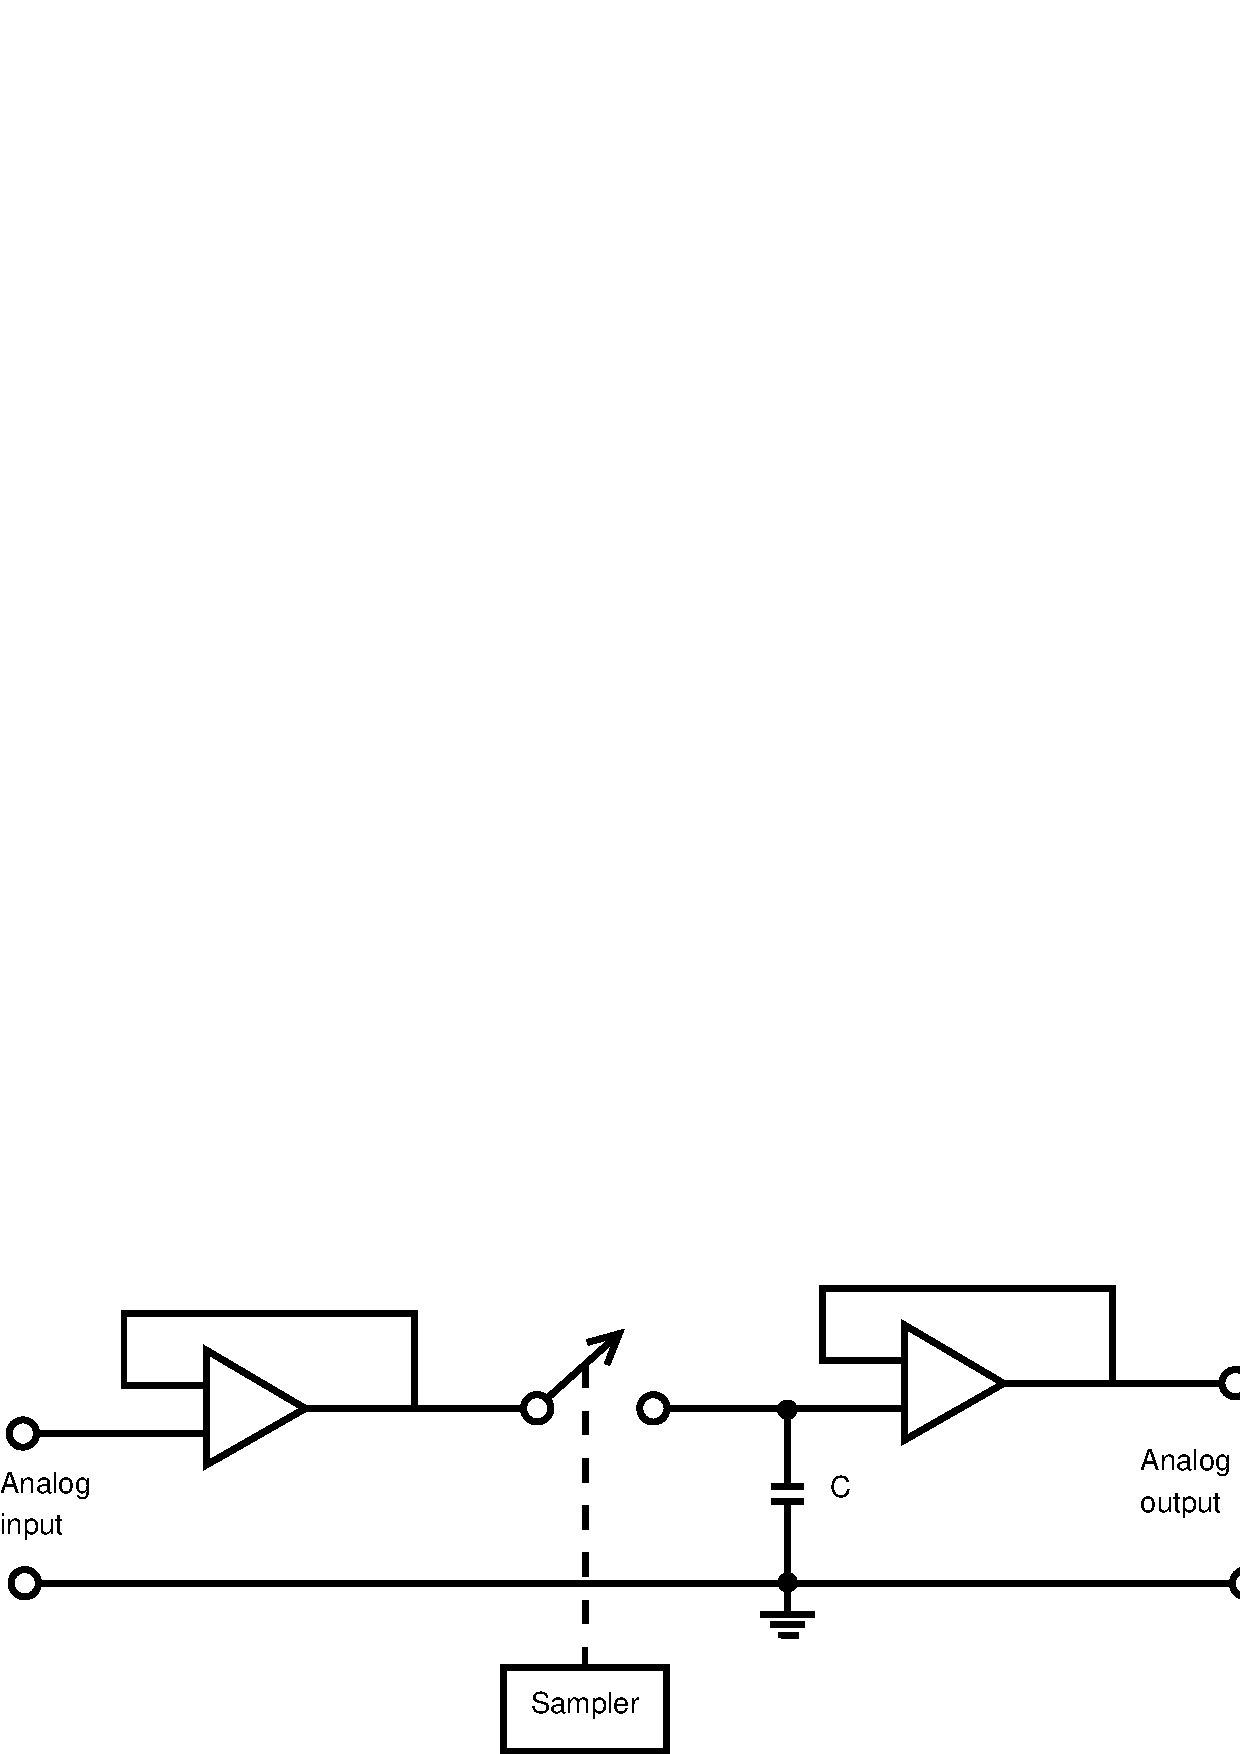
\includegraphics[width=0.8\linewidth]{sample_hold}
	\end{figure}
	\vspace{-2ex}
	When the switch is closed, the input signal is connected and the circuit is in \textbf{tracking mode}. The charge on the capacitor in the circuit tracks the input voltage.\\
	When the switch is open, the input signal is disconnected and the circuit is in \textbf{hold mode}. The capacitor voltage holds constant for a specified time period.
\end{frame}

\begin{frame}
	\frametitle{A/D converter}
	\begin{figure}
		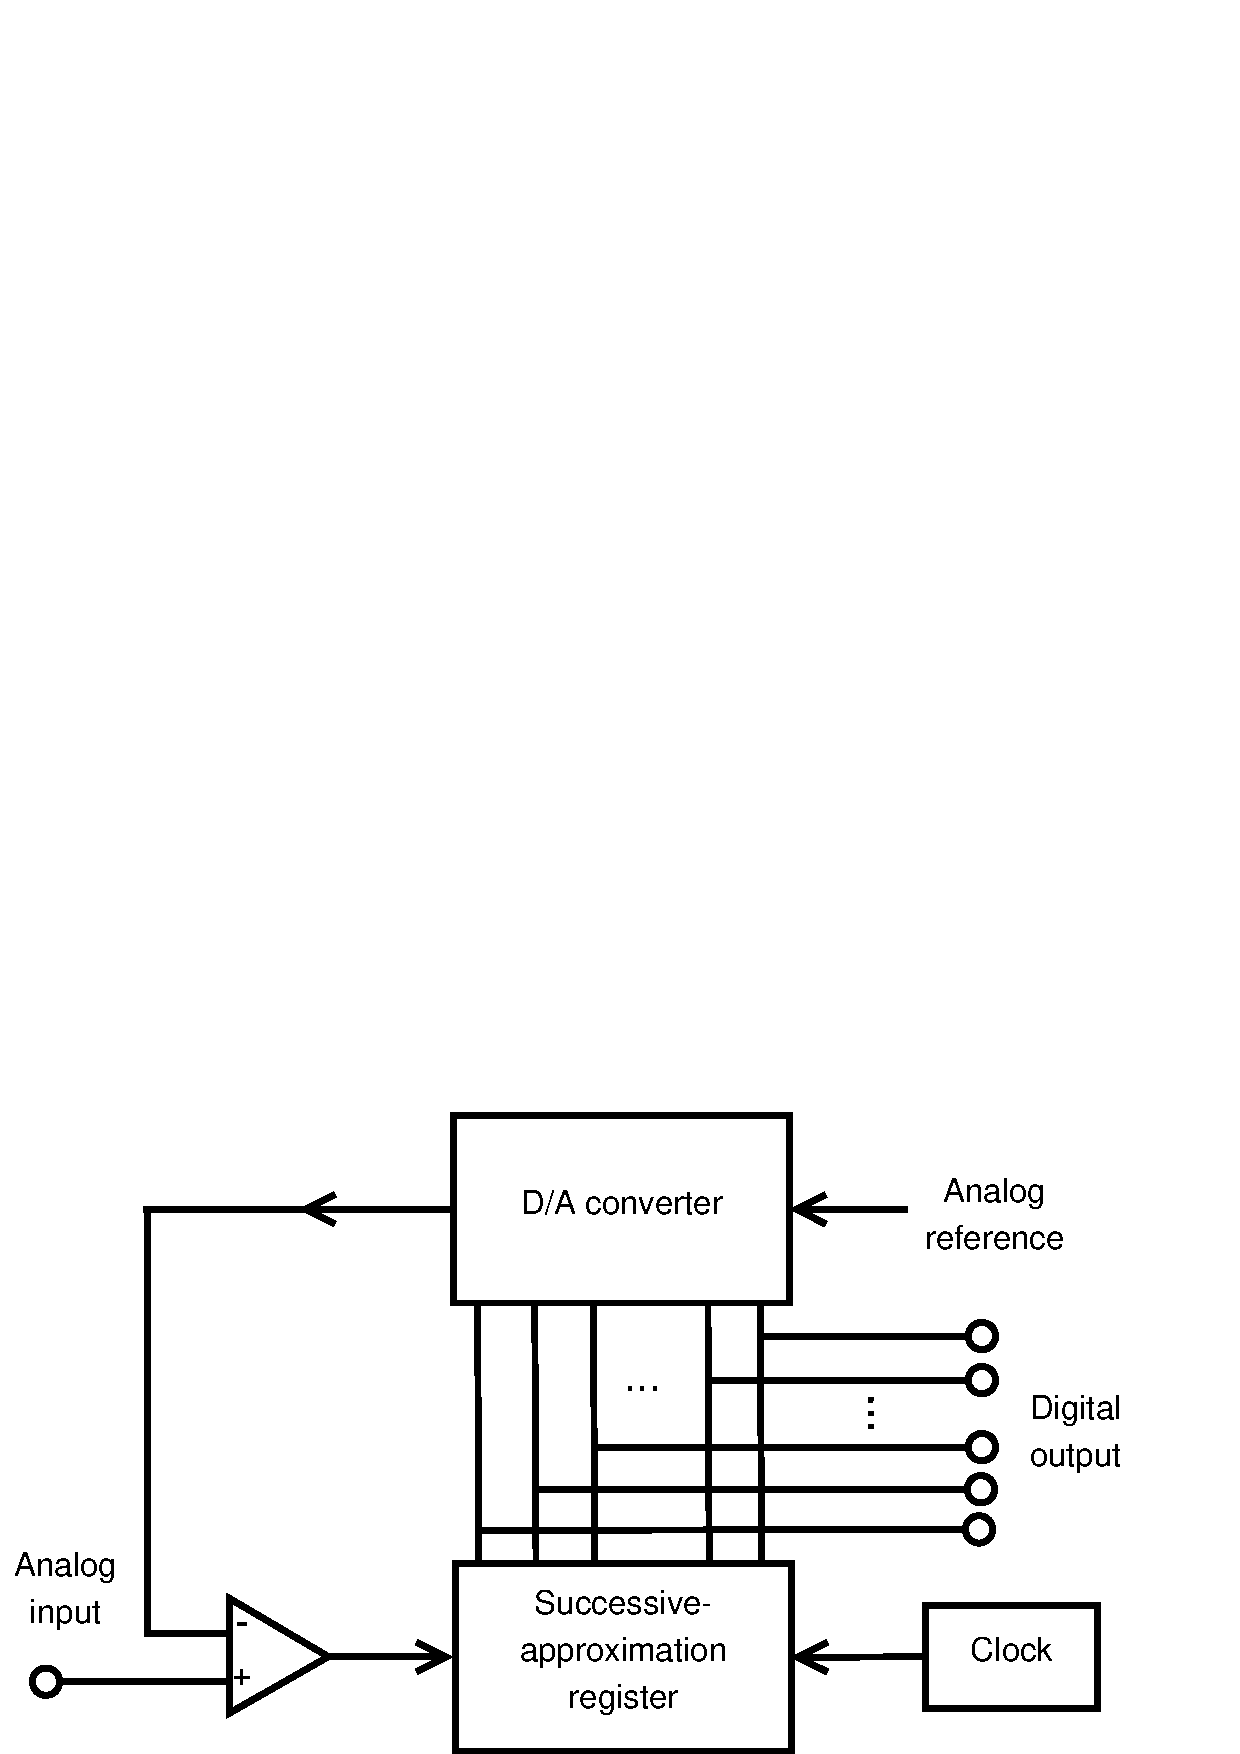
\includegraphics[width=0.6\linewidth]{ADconverter}
	\end{figure}
	The successive-approximation register (SAR) is most frequently used. It turns on the most significant bit and compares it with the analog input. The comparator decides whether to leave the bit on or turn it off (if the analog input voltage is larger, the most significant bit is set on). Then the register continues with bit 2.
\end{frame}

\begin{frame}
	\frametitle{A/D converter}
	\begin{figure}
		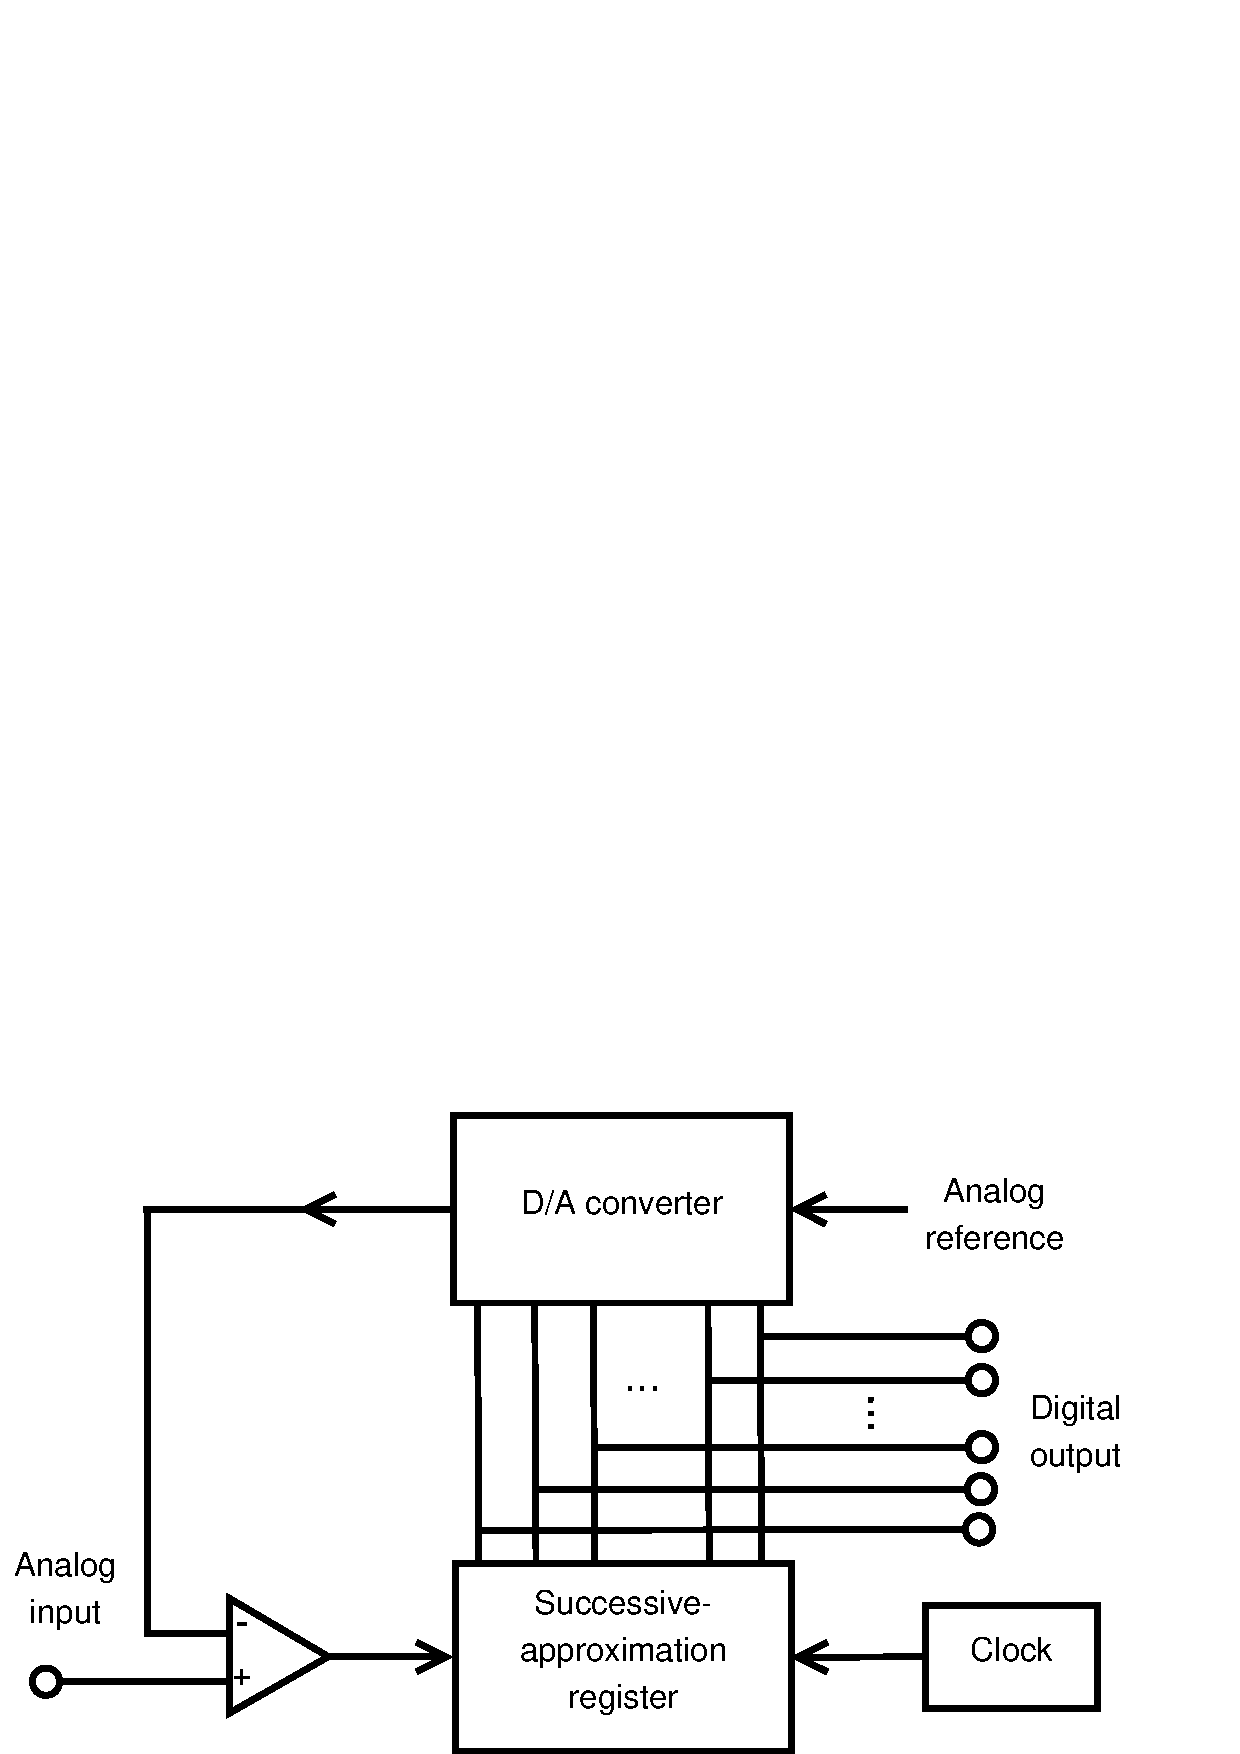
\includegraphics[width=0.8\linewidth]{ADconverter}
	\end{figure}
	After n comparisons, the digital output of the register indicates all those bits that remain on and produces the desired digital code.
\end{frame}

\begin{frame}
	\frametitle{D/A converter}
	\vspace{-4ex}
	\begin{figure}
		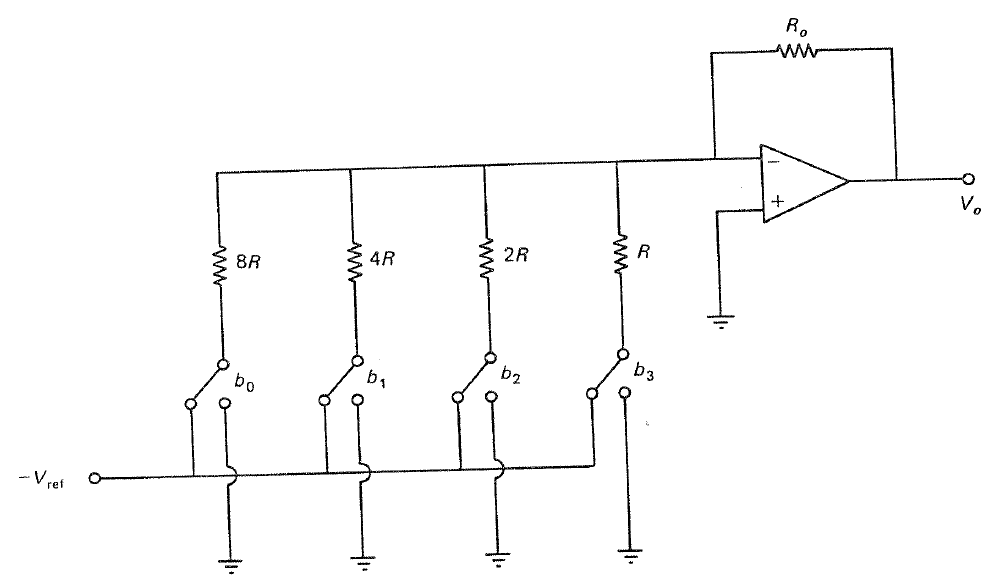
\includegraphics[width=0.8\linewidth]{DAconverter}
	\end{figure}
	The input resistor of the operational amplifier have their resistance values weighted in a binary fashion. 
\end{frame}

\begin{frame}
	\frametitle{D/A converter}
	\vspace{-2ex}
	\begin{figure}
		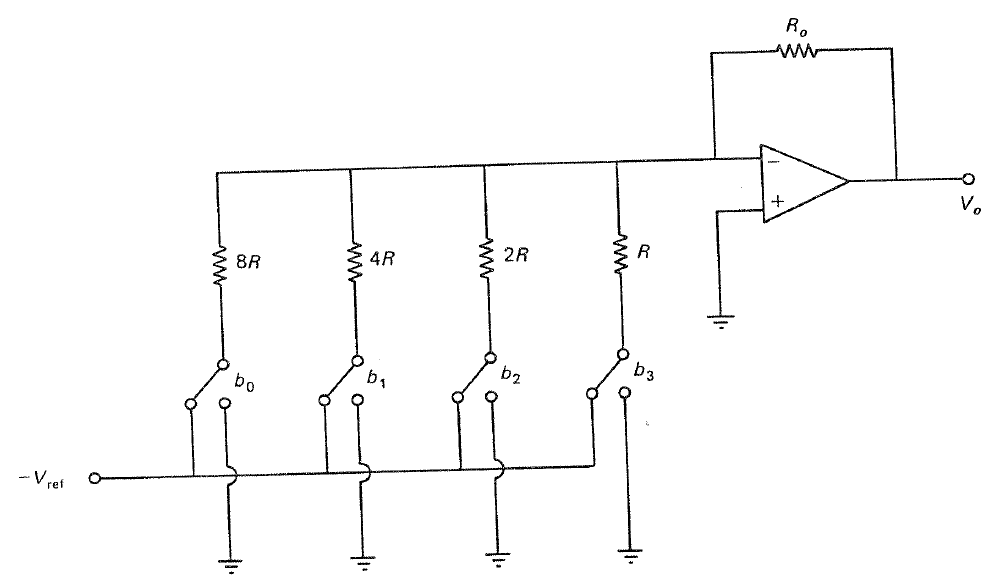
\includegraphics[width=0.8\linewidth]{DAconverter}
	\end{figure}
	When the logic circuit receives binary 1, the switch connects the resistor to the reference voltage. When the logic circuit receives binary 0, the switch connects the resistor to ground.
\end{frame}

\begin{frame}
	\frametitle{D/A converter}
	\vspace{-3ex}
	\begin{figure}
		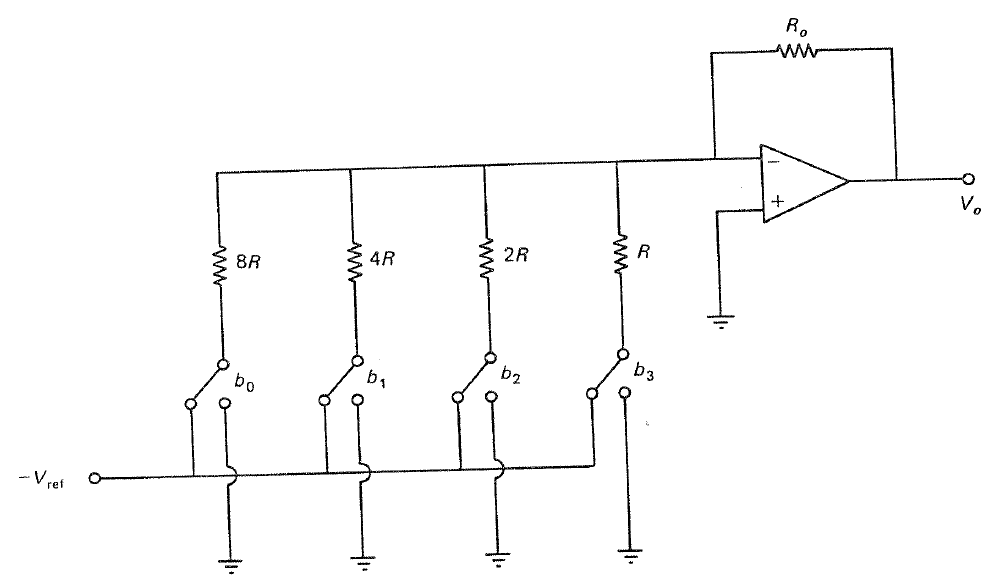
\includegraphics[width=0.8\linewidth]{DAconverter}
	\end{figure}
	If the binary number (here) is $b_3b_2b_1b_0$, each of the b's can be 0 or 1, the output is $V_o = \frac{R_o}{R} \Big(b_3+\frac{b_2}{2} + \frac{b_1}{4}+\frac{b_0}{8}\Big) V_{ref}$
\end{frame}

\section{Analysis of the sample and hold}

\begin{frame}
	\frametitle{Analysis of the sample and hold}
	To get samples of a continuous signal, we use an analog-to-digital converter. The conversion always takes a non-zero time.\\
	\vspace{1em}
	To give the computer an accurate representation of the signal exactly at the sampling instants $kT_s$, the converter is preceded by a sample-and-hold circuit.\\
	\vspace{1em}
	The sample-and-hold will take the impulses that are produced by the mathematical sampler and produce the piecewise constant output of the device.
\end{frame}

\begin{frame}
	\frametitle{Sampling operation}
	\begin{block}{}
	The sampling operation is represented by impulse modulation. Its role is to give a mathematical representation of taking periodic samples from $r(t)$ to produce $r(kT_s)$. \\
	\vspace{1em}
	The sampler takes as input $r(t)$ and returns as output
	\begin{center}
	$r^*(t)=\sum_{k=-\infty}^{\infty} r(t)\delta(t-kT_s)$.
	\end{center}
	\vspace{1em}
	The Laplace transform of $r^*(t)$ can be computed as\\
	\vspace{-1.5em}
	\begin{align*} 
	\mathcal{L}\{r^*(t)\} = \int_{-\infty}^{\infty} r^*(\tau)e^{-s\tau} d\tau = \int_{-\infty}^{\infty} \sum_{k=-\infty}^{\infty} r(\tau)\delta(\tau-kT_s)e^{-s\tau}d\tau 
	\end{align*}\\
	\end{block}
\end{frame}

\begin{frame}
	\frametitle{Sampling operation}
	\begin{block}{}
	Using $\int_{-\infty}^{\infty} f(t)\delta(t-a)dt = f(a)$ we obtain \\ 
	\begin{center}
		$\mathcal{L}\{r^*(t)\} = R^*(s) = \sum_{k=-\infty}^{\infty} r(kT_s)e^{-skT_s}$
	\end{center}
	\end{block}
	\vspace{1em}
	\begin{columns}
		\begin{column}{0.5\textwidth}
			If the signal r(t) is shifted a small amount, then different samples will be selected by the sampling process for the output, proving that sampling is not a time-invariant process.
		\end{column}
		\begin{column}{0.5\textwidth}
			\begin{figure}
				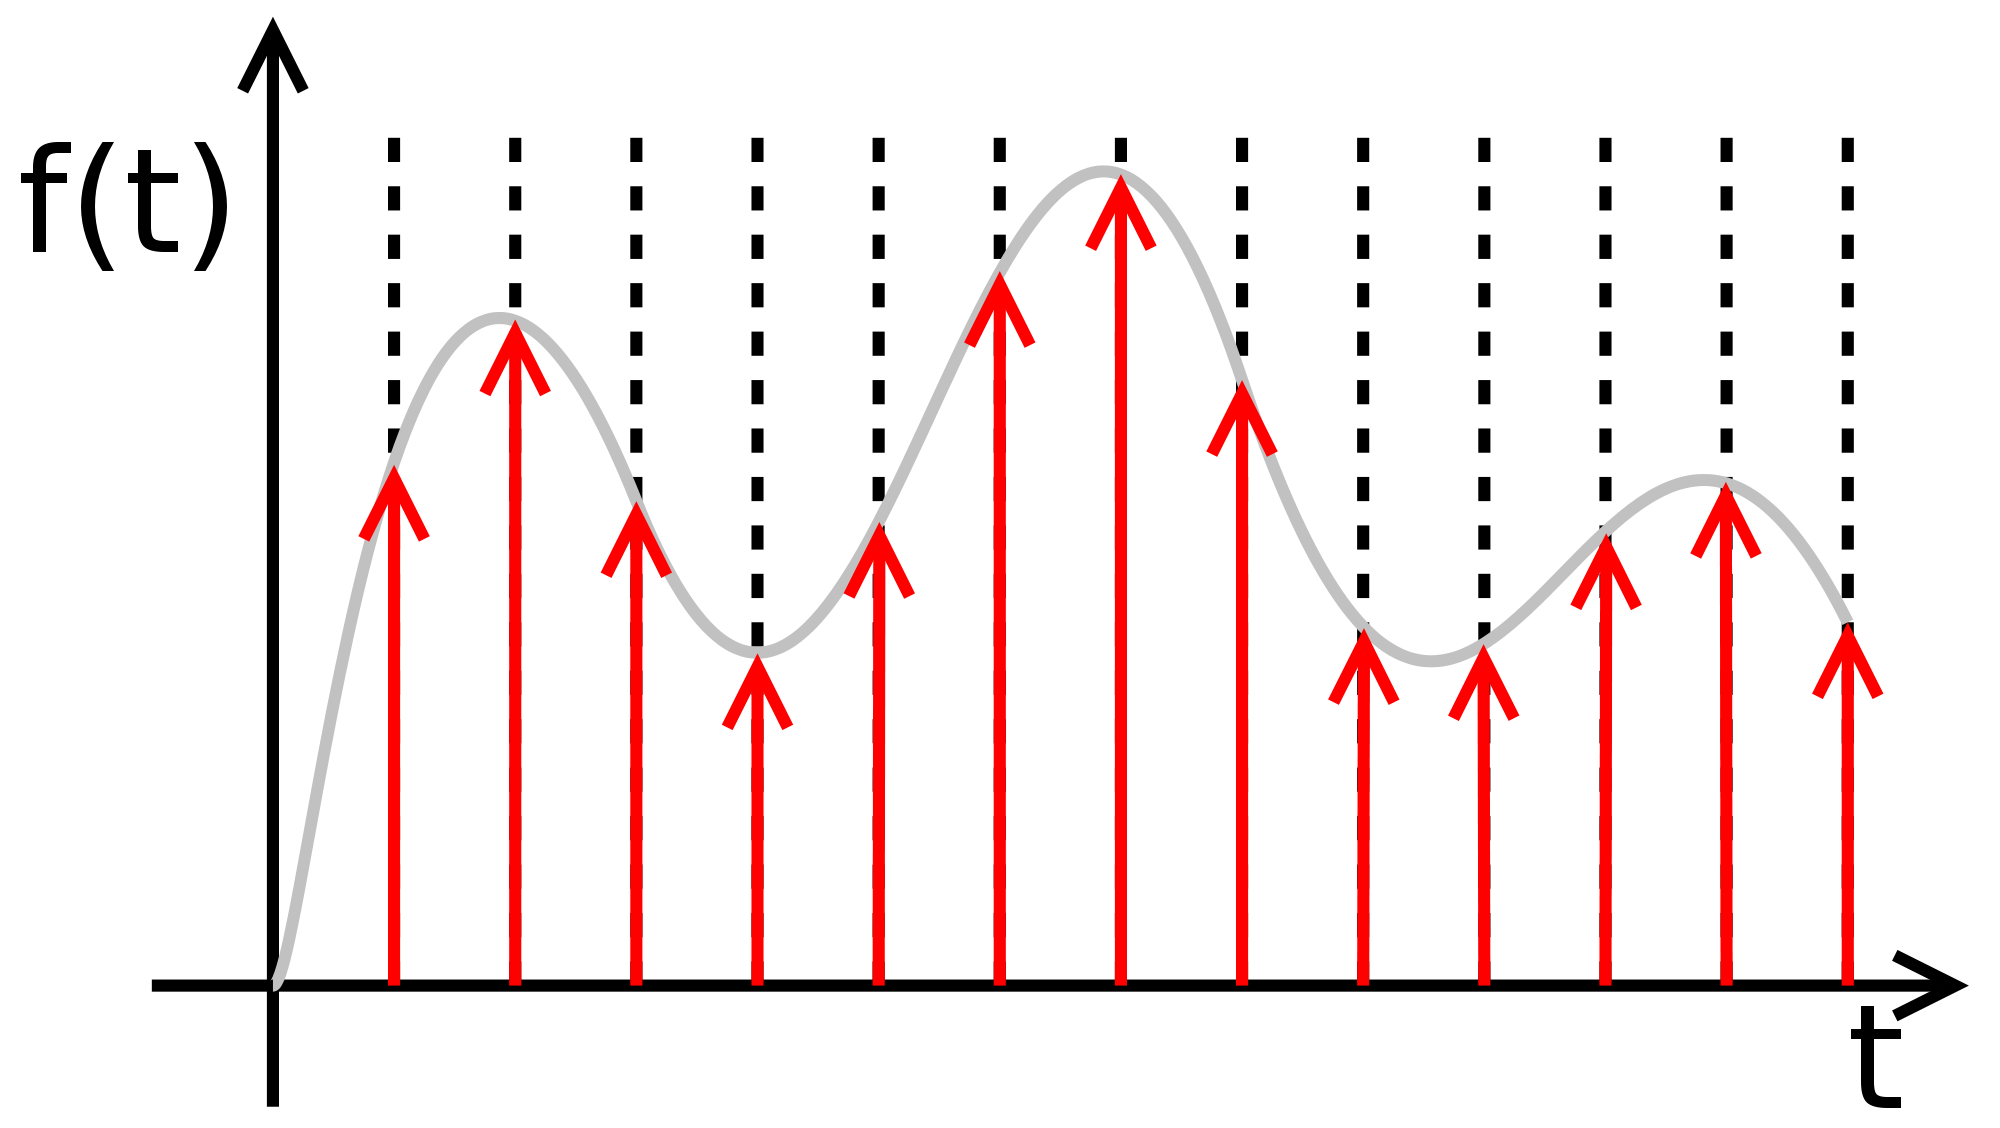
\includegraphics[width=0.9\linewidth]{sampled_signal}
			\end{figure}	
		\end{column}	
	\end{columns}
	%source: https://commons.wikimedia.org/wiki/File:Sampled.signal.svg
\end{frame}

\begin{frame}
	\frametitle{Hold operation}
	\begin{block}{}
	The hold operation is represented as a linear filter. It is defined by means whereby the impulses are extrapolated to the piecewise constant signal $r_h(t) = r(kT_s)$ with $kT_s \leq t < (k+1)T_s$.\\
	\end{block}
	\vspace{1em}
	\begin{columns}
		\begin{column}{0.5\textwidth}
		A general technique is to use a polynomial fit to the past samples.If the extrapolation is done by a constant (a zero-order polynomial), then the extrapolator is called a zero-order hold and its transfer function is denoted $ZOH(s)$. 
		\end{column}
		\begin{column}{0.5\textwidth}
		\begin{figure}
			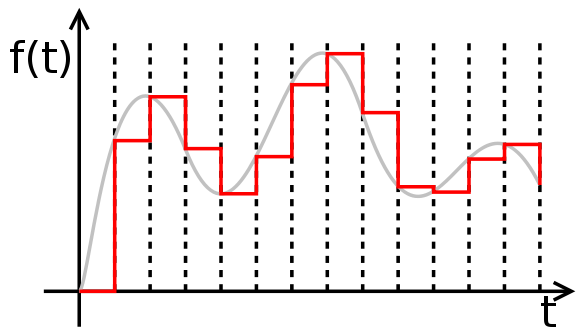
\includegraphics[width=1\linewidth]{sample_and_hold}
		\end{figure}	
		\end{column}	
	\end{columns}
	%source: https://en.wikipedia.org/wiki/Sample_and_hold#/media/File:Zeroorderhold.signal.svg
\end{frame}

\begin{frame}
	\frametitle{Zero-order hold}
	We compute the transfer function as the transform of its impulse response. If $r^*(t)=\delta(t)$ then $r_h(t)$ is a pulse of height 1 and duration T: $r_h(t) = 1(t) - 1(t-T_s)$. Which has the following Laplace transform:\\
	\vspace{-0.5em}
	\begin{center}
		$ZOH(s)=\mathcal{L}\{p(t)\} = \int_{0}^{\infty} [1(t)-1(t-T_s)]e^{-s\tau}d\tau = \frac{1-e^{-sT_s}}{s}$
	\end{center}
	\vspace{-1.3em}
	\begin{figure}
		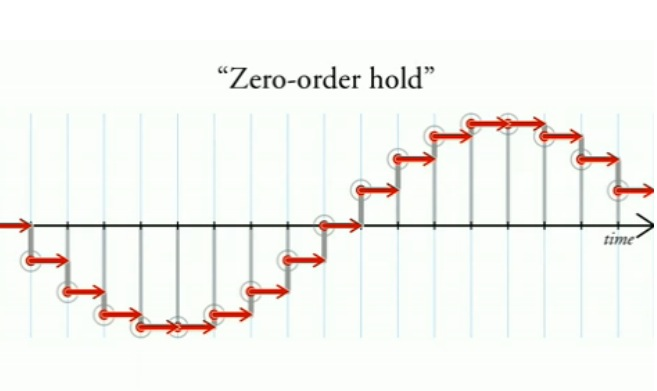
\includegraphics[width=0.6\linewidth]{zoh}
	\end{figure}
	%source: http://www.audiorecordingschool.com/blog/chris-montgomery-explains-digital-audio/
\end{frame}

\section{Fourier transform}

\begin{frame}
	\frametitle{Fourier transform}
	\begin{center}
		\Large{
		$f(t)\xrightarrow{\qquad \qquad \qquad \qquad \qquad \qquad \qquad \qquad}F(j\omega)$\\
		$F(j\omega) = \int_{-\infty}^{\infty} f(t)e^{-j\omega t} dt$\\
		\bigskip
		$f(t)\xleftarrow{\qquad \qquad \qquad \qquad \qquad \qquad \qquad \qquad}F(j\omega)$\\
		$f(t) = \frac{1}{2\pi} \int_{-\infty}^{\infty} F(j\omega) e^{j\omega t} d\omega$}
	\end{center}
\end{frame}

\begin{frame}
	\frametitle{Fourier transform}
	\begin{figure}
		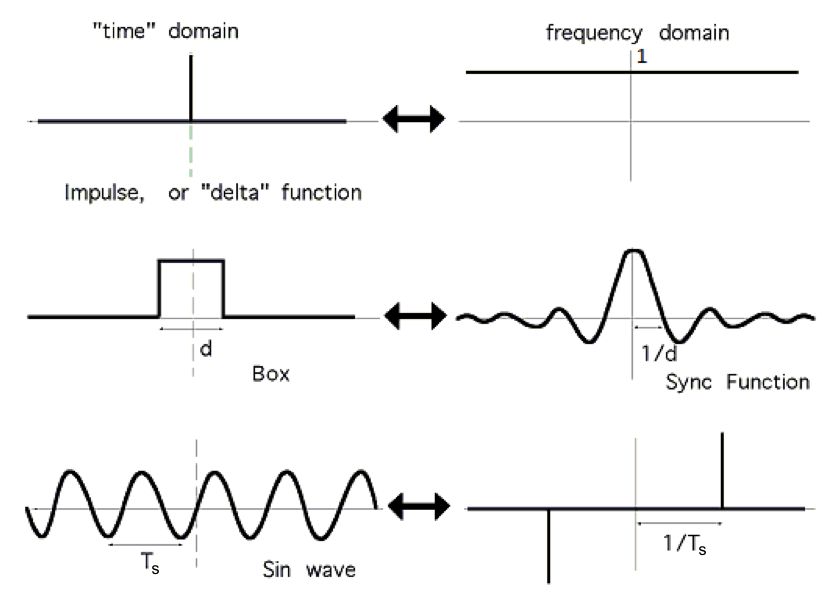
\includegraphics[width=.8\linewidth]{fourier_examples}
	\end{figure}
\end{frame}

\begin{frame}
	\frametitle{Fourier transform: properties}
	\begin{itemize}
		\item \textbf{Linearity} \\
		\vspace{-3ex}
		\begin{align*}
		& \begin{cases}
		f_1(t) \leftrightarrow F_1(j\omega)\\
		f_2(t) \leftrightarrow F_2(j\omega)
		\end{cases} && \Rightarrow \quad a f_1(t) + b f_2(t) \leftrightarrow a F_1(j\omega) + b F_2(j \omega)
		\end{align*}
		\item \textbf{Time-scaling} \\
		\medskip
		$f(a t) \leftrightarrow (\frac{1}{|a|}) F(\frac{j \omega}{a})$
		\medskip
		\item \textbf{Translation/Time-shifting} \\
		\medskip
		$f (t - t_0) \leftrightarrow e^{-j \omega t_0} F(j\omega)$
		\medskip
		\item \textbf{Modulation/Frequency-shifting} \\
		\medskip
		$e^{j \omega_0 t} f(t) \leftrightarrow F(j (\omega - \omega_0))$
	\end{itemize}
\end{frame}

\begin{frame}
	\frametitle{Fourier transform: properties}
	\begin{itemize}
		\item \textbf{Reciprocity} \\
		\medskip
		$F(-jt) \leftrightarrow  2 \pi f(\omega)$
		\medskip
		\item \textbf{Derivative in t} \\
		\medskip
		$\frac{df(t)}{dt} \leftrightarrow j\omega F(j\omega) \qquad \qquad \quad \frac{d^nf(t)}{dt^n} \leftrightarrow (j\omega)^n F(j\omega)$
		\medskip
		\item \textbf{Derivative in $\omega$} \\
		\medskip
		$(-jt)^n f(t) \leftrightarrow \frac{d^n F(j\omega)}{d\omega^n} \qquad \quad \frac{f(t)}{-jt} \leftrightarrow \int_{-\infty}^\infty F(j\Omega) d\Omega \> if \> f(0) = 0$
		\medskip
		\item \textbf{Convolution} \\
		\medskip
		$y(t) = h(t) * u(t) \leftrightarrow Y(j\omega) = H(j\omega) U(j\omega)$\\
		$v(t) = h(t)u(t) \leftrightarrow V(j\omega) = \frac{1}{2\pi} H(j\omega)*U(j\omega)$
	\end{itemize}
\end{frame}

\section{Spectrum of a sampled signal}

\begin{frame}
	\frametitle{Spectrum of a sampled signal}
	$r^*(t)$ is the product of $r(t)$ and a train of impulses. The latter series is periodic and can be represented by a Fourier series:\\
	\begin{center}
		$\sum_{k=-\infty}^{\infty} \delta(t-kT_s) = \sum_{n=-\infty}^{\infty} C_ne^{j(2\pi n/T_s)}t$,
	\end{center}
	where the Fourier coefficients $C_n$ are given by:\\
	\begin{center}
		$C_n=\frac{1}{T_s}\int_{-T_s/2}^{T_s/2} \sum_{k=-\infty}^{\infty} \delta(t-kT_s)e^{-jn(2\pi t/T_s)}dt$.
	\end{center}
	
\end{frame}

\begin{frame}
	\frametitle{Spectrum of a sampled signal}
	The only term in the sum of impulses that is in the range of the integral is the $\delta(t)$ at the origin, so the integral reduces to: \\
	\begin{center}
		$C_n=\frac{1}{T_s}\int_{-T_s/2}^{T_s/2}\delta(t)e^{-jn(2\pi t/T_s)}dt=\frac{1}{T_s}$.
	\end{center}
	We derived the Fourier series of the sum of impulses:\\
	\begin{center}
		$\sum_{k=-\infty}^{\infty} \delta(t-kT_s)=\frac{1}{T_s}\sum_{n=-\infty}^{\infty} e^{j(2\pi n/T_s)t}$.
	\end{center}
	We define $\omega_s = \frac{2\pi}{T_s}$ as the sampling frequency (rad/s).\\
\end{frame}

\begin{frame}
	\frametitle{Spectrum of a sampled signal}
	We take the Laplace transform of the output of the sampler,
	\vspace{-1em}
	\begin{center}
		\begin{equation}
			\begin{split}
			R^*(s)& = \int_{-\infty}^{\infty} r(t) \Big\{ \frac{1}{T_s} \sum_{n=-\infty}^{\infty} e^{jn\omega_st} \Big\} e^{-st} dt\\
			& = \frac{1}{T_s} \sum_{n=-\infty}^{\infty} \int_{-\infty}^{\infty} r(t) e^{jn\omega_st}e^{-st}dt\\
			& = \frac{1}{T_s} \sum_{n=-\infty}^{\infty} \int_{-\infty}^{\infty}r(t) e^{-(s-jn\omega_s)t} dt.
			\end{split}
		\end{equation}
	\end{center}
\end{frame}

\begin{frame}
	\frametitle{Spectrum of a sampled signal}
	\begin{definition}
	Since the integral is the Laplace transform of $r(t)$ with only a change of variable where the frequency goes, the result can be written as:\\
	\begin{center}
		$R^*(s)=\frac{1}{T_s}\sum_{n=-\infty}^{\infty}R(s-jn\omega_s)$.
	\end{center}
	\end{definition}
\end{frame}

\subsection{Aliasing}

\begin{frame}
	\frametitle{Aliasing}
	\begin{definition}
	Aliasing is	an effect that causes different signals to become indistinguishable when sampled. Frequencies that are too high to be sampled are folded onto lower frequencies. We cannot distinguish them based on their samples alone.
	\end{definition}
\end{frame}

\begin{frame}
	\frametitle{Aliasing}
	\begin{example}
	The red sine wave is being sampled at just over its bandwidth, however the blue sine wave will be recreated as it also fits all data points and is within the expected bandwidth.
	\vspace{-0.7em}
	\begin{figure}
		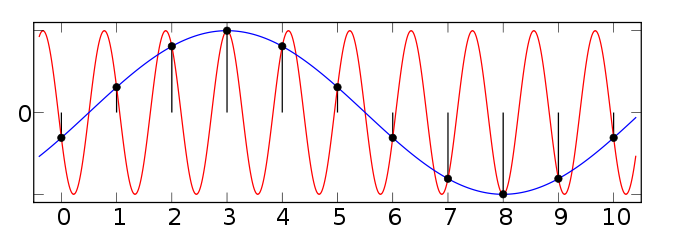
\includegraphics[width=1\linewidth]{aliasing}
	\end{figure}
	%source: https://en.wikipedia.org/wiki/Aliasing#/media/File:AliasingSines.svg
	\end{example}
\end{frame}

\begin{frame}
	\frametitle{Aliasing}
	As a direct result of the sampling operation, when data is sampled at a frequency $\frac{2\pi}{T_s}$, the total harmonic content at a given frequency $\omega_1$ is to be found not only from the original signal at $\omega_1$, but also from all those frequencies that are aliases of $\omega_1$, namely $\omega_1 + n2\pi/T_s = \omega_1+n\omega_s$.\\
	\vspace{1em}
	The errors caused by aliasing can be very severe if a substantial quantity of high-frequency components is contained in the signal to be sampled. To minimize this error, the sampling operation is preceded by a low-pass anti-aliasing filter that will remove all spectral content above the half-sampling frequency ($\pi/T_s$).
\end{frame}

\subsection{Sampling theorem}

\begin{frame}
	\frametitle{Shannon-Nyquist sampling theorem}
	\begin{block}{}
	If all content above the half-sampling frequency is removed, no aliasing is introduced by sampling. Also the signal spectrum is not distorted, even though it is repeated endlessly, centered at $n2\pi/T_s$.\\
	\medskip
	This critical frequency, $\pi/T_s$, is called the \textbf{Nyquist frequency}. Band-limited signals that have no components above the Nyquist frequency are represented unambiguously by their samples. \\
	\medskip
	This is the \textbf{sampling theorem}: One can recover a signal from its samples if the sampling frequency ($\omega_s=2\pi/T_s$) is at least twice the highest frequency ($\pi/T$) in the signal. This maximum frequency is also called the \textbf{bandwidth} B.
	\end{block}
\end{frame}

\begin{frame}
	\frametitle{Shannon-Nyquist sampling theorem}
	\begin{columns}
		\begin{column}{0.5\textwidth}
		The signal can be fully reconstructed if there are no overlaps in the frequency domain.\\
		If the sampling frequency is at least twice the bandwidth B, then the signal can be reconstructed without a problem (no overlap). (fig. a)\\
		If the sampling frequency is too low then information will be lost (overlap). (fig. b)\\
		\begin{alertblock}{}
		\textbf{Sampling frequency} $f_s \geq 2 B$
		\end{alertblock}
		\end{column}
		\begin{column}{0.5\textwidth}
		\begin{figure}
			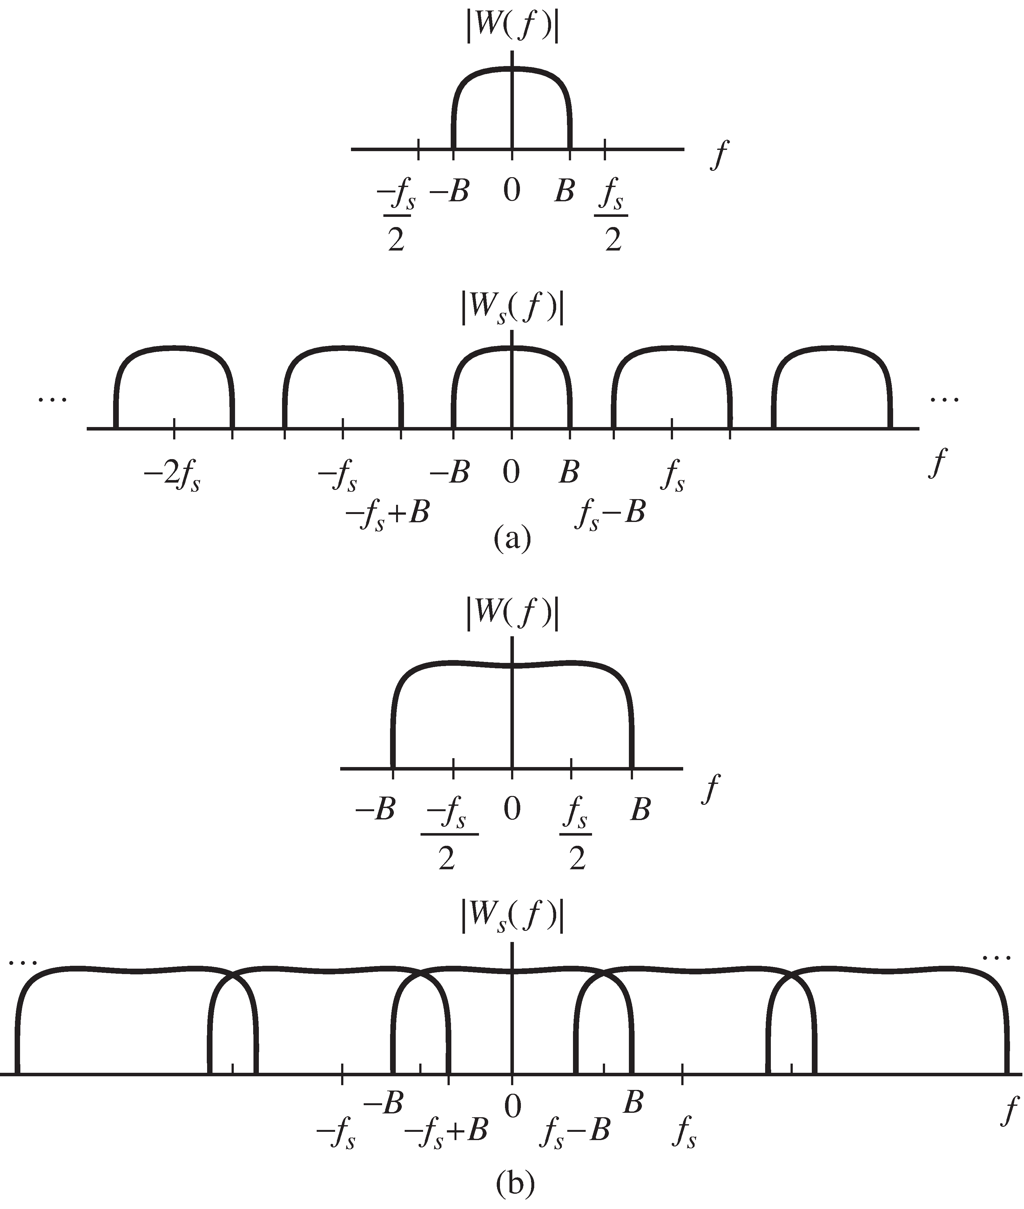
\includegraphics[width=0.9\linewidth]{nyquist}
		\end{figure}
		\end{column}
	\end{columns}
\end{frame}

\subsection{Hidden oscillations}

\begin{frame}
	\frametitle{Hidden oscillations}
	\begin{definition}
	There is the possibility that a signal contains some frequencies that the samples do not show at all. \\
	\vspace{1em}
	Such signals, when they occur in digital control systems, are called \textbf{hidden oscillations}.\\
	\vspace{1em}
	They can only occur at multiples of the Nyquist frequency ($\pi/T_s$).
	\end{definition}
\end{frame}

\section{Data extrapolation (reconstruction)}

\begin{frame}
	\frametitle{Reconstruction}
	\begin{columns}
		\begin{column}{0.4\textwidth}
		\underline{\smash{Sampling theorem}}: \textit{under the right conditions} it is possible to recover a signal from its samples.\\
		\vspace{1em}
		The figure to the right shows the spectrum of $R(j\omega)$. It is contained in the low-frequency part of $R^*(j\omega)$. Therefore, to recover $R(j\omega)$ we need to process $R^*(j\omega)$ through a low-pass filter and multiply by $T_s$.\\
		\end{column}
		\begin{column}{0.6\textwidth}
		\vspace{-4ex}
		\begin{figure}
			\centering
			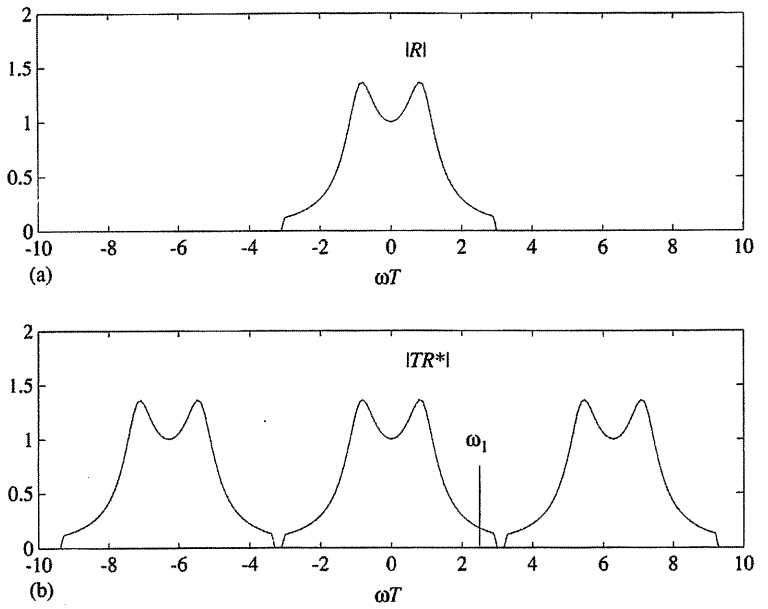
\includegraphics[width=1\linewidth]{reconstruction}
		\end{figure}
		\end{column}
	\end{columns}
\end{frame}

\begin{frame}
	\frametitle{Reconstruction}
	If $R(j\omega)$ has zero energy for frequencies in the bands above the Nyquist frequency, in other words R is band-limited, then an ideal low-pass filter with gain T for $-\pi/T \leq \omega \leq \pi/T$ and zero elsewhere would recover $R(j\omega)$ from $R^*(j\omega)$ exactly.\\
	\medskip
	If we define the ideal low-pass filter characteristic as $L(j\omega)$, we have:
	\begin{center}
		$R(j\omega)=L(j\omega)R^*(j\omega)$.
	\end{center}
	The signal $r(t)$ is the inverse Fourier transform of $R(j\omega)$. Because $R(j\omega)$ is the \textit{product} of two Fourier transforms, $r(t)$ is the \textit{convolution} of the time functions $\ell(t)$ and $r^*(t)$.\\
	\begin{center}
		$r(t) = \ell(t) * r^*(t)$.
	\end{center}
\end{frame}

\begin{frame}
	\frametitle{Ideal low-pass filter}
	The impulse response of the filter can be computed using this definition:\\
	\vspace{-1em}
	\begin{equation}
	\begin{split}
	\ell(t) & = \frac{1}{2\pi} \int_{-\pi/T_s}^{\pi/T_s}Te^{j\omega t}d\omega\\
	& = \frac{T_s}{2\pi} \frac{e^{j\omega t}}{jt} \Big|_{-\pi/T_s}^{\pi/T_s}\\
	& = \frac{T_s}{2\pi jt}(e^{j(\pi t/T_s)}-e^{-j(\pi t/T_s)})\\
	& = \frac{sin(\pi t/T_s)}{\pi t/T_s}\\
	& \triangleq sinc\frac{\pi t}{T_s} \nonumber
	\end{split}
	\end{equation}
\end{frame}

\begin{frame}
	\frametitle{Ideal low-pass filter}
	The sinc functions are the interpolators that fill in the time gaps between samples with a signal that has no frequencies above $\pi/T_s$.
	\begin{figure}
		\centering
		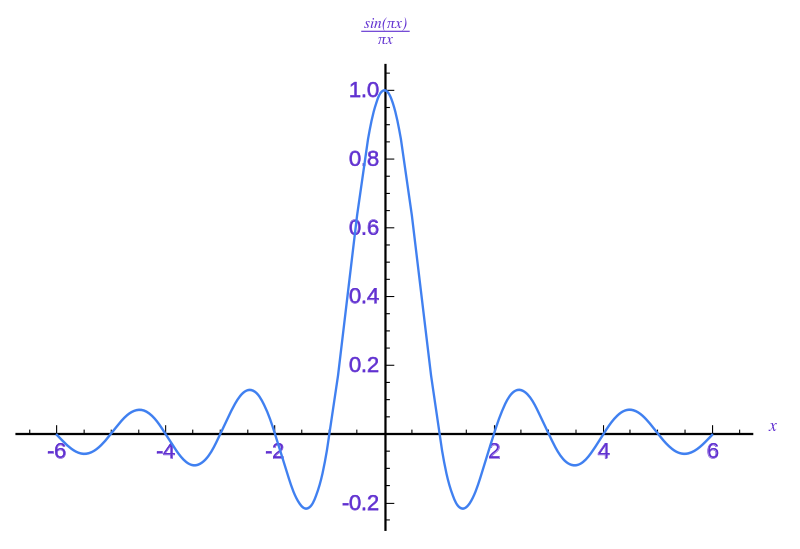
\includegraphics[width=0.7\linewidth]{sinc}
	\end{figure}
	%source: https://en.wikipedia.org/wiki/Rectangular_function#/media/File:Sinc_function_(normalized).svg
\end{frame}

\begin{frame}
	\frametitle{Reconstruction}
	\begin{block}{}
	Using the previous equations, we find:\\
	\begin{center}
	$r(t)=\int_{-\infty}^{\infty} r(\tau)\sum_{k=-\infty}^{\infty} \delta(\tau-kT_s)sinc\frac{\pi(t-\tau)}{T_s}d\tau.$
	\end{center}
	Using the shifting property of the impulse, we obtain:
	\begin{center}
	${r(t)=\sum_{k=-\infty}^{\infty} r(kT_s)sinc\frac{\pi(t-kT_s)}{T_s}}$.
	\end{center}
	\end{block}
	\begin{alertblock}{}
	This filter is non-causal because $\ell(t)$ is nonzero for $t < 0$. $\ell(t)$ starts at $t=-\infty$ while the impulse that triggers it does not occur until $t=0$. The non-causality can be overcome by adding a phase lag, $e^{-j\omega \lambda}$, to $L(j\omega)$, which adds a delay to the filter and to the signals processed through it.
	\end{alertblock}
\end{frame}

\begin{frame}
	\frametitle{Zero-order hold}
	The transfer function of the zero-order hold was introduced as\\
	\vspace{-1ex}
	\begin{center}
		$ZOH(j\omega)=\frac{1-e^{-j\omega T_s}}{j\omega}$.\\
	\end{center}
	\vspace{-1ex}
	We express this function in magnitude and phase form, to discover the frequency properties of $ZOH(j\omega)$.\\
	\medskip
	We factor out $e^{-j\omega T_s/2}$ and multiply and divide by $2j$:\\
	\vspace{-4ex}
	\begin{equation}
	\begin{split}
		ZOH(j\omega) &= e^{-j\omega T_s/2}\Big\{\frac{e^{j\omega T_s/2}-e^{-j\omega T_s/2}}{2j}\Big\} \frac{2j}{j\omega}\\
		& = T_se^{-j\omega T_s/2} \frac{sin(\omega T_s/2)}{\omega T_s/2}\\
		& = e^{-j\omega T_s/2} T_s sinc(\omega T_s/2)
	\end{split} \nonumber
	\end{equation}
	\vspace{-1ex}
\end{frame}

\begin{frame}
	\frametitle{Zero-order hold}
	The magnitude function is\\
	\vspace{-1ex}
	\begin{center}
		$|ZOH(j\omega)| = T_s\Big|sinc\frac{\omega T_s}{2} \Big|$
	\end{center}
	\vspace{-1ex}
	and the phase is\\
	\vspace{-1ex}
	\begin{center}
		$\angle ZOH(j\omega)=\frac{-\omega T_s}{2}$
	\end{center}
	\vspace{-1ex}
	plus the $180^\circ$ shifts where the sinc function changes sign.\\
	\vspace{1em}
	Thus the effect of the zero-order hold is to introduce a phase shift of $\omega T_s/2$ (a time delay of $T_s/2$ seconds) and to multiply the gain by a function with the magnitude of $sinc(\omega T_s/2)$.
\end{frame}

\begin{frame}
	\frametitle{Zero-order hold filter vs ideal filter}
	\begin{figure}
		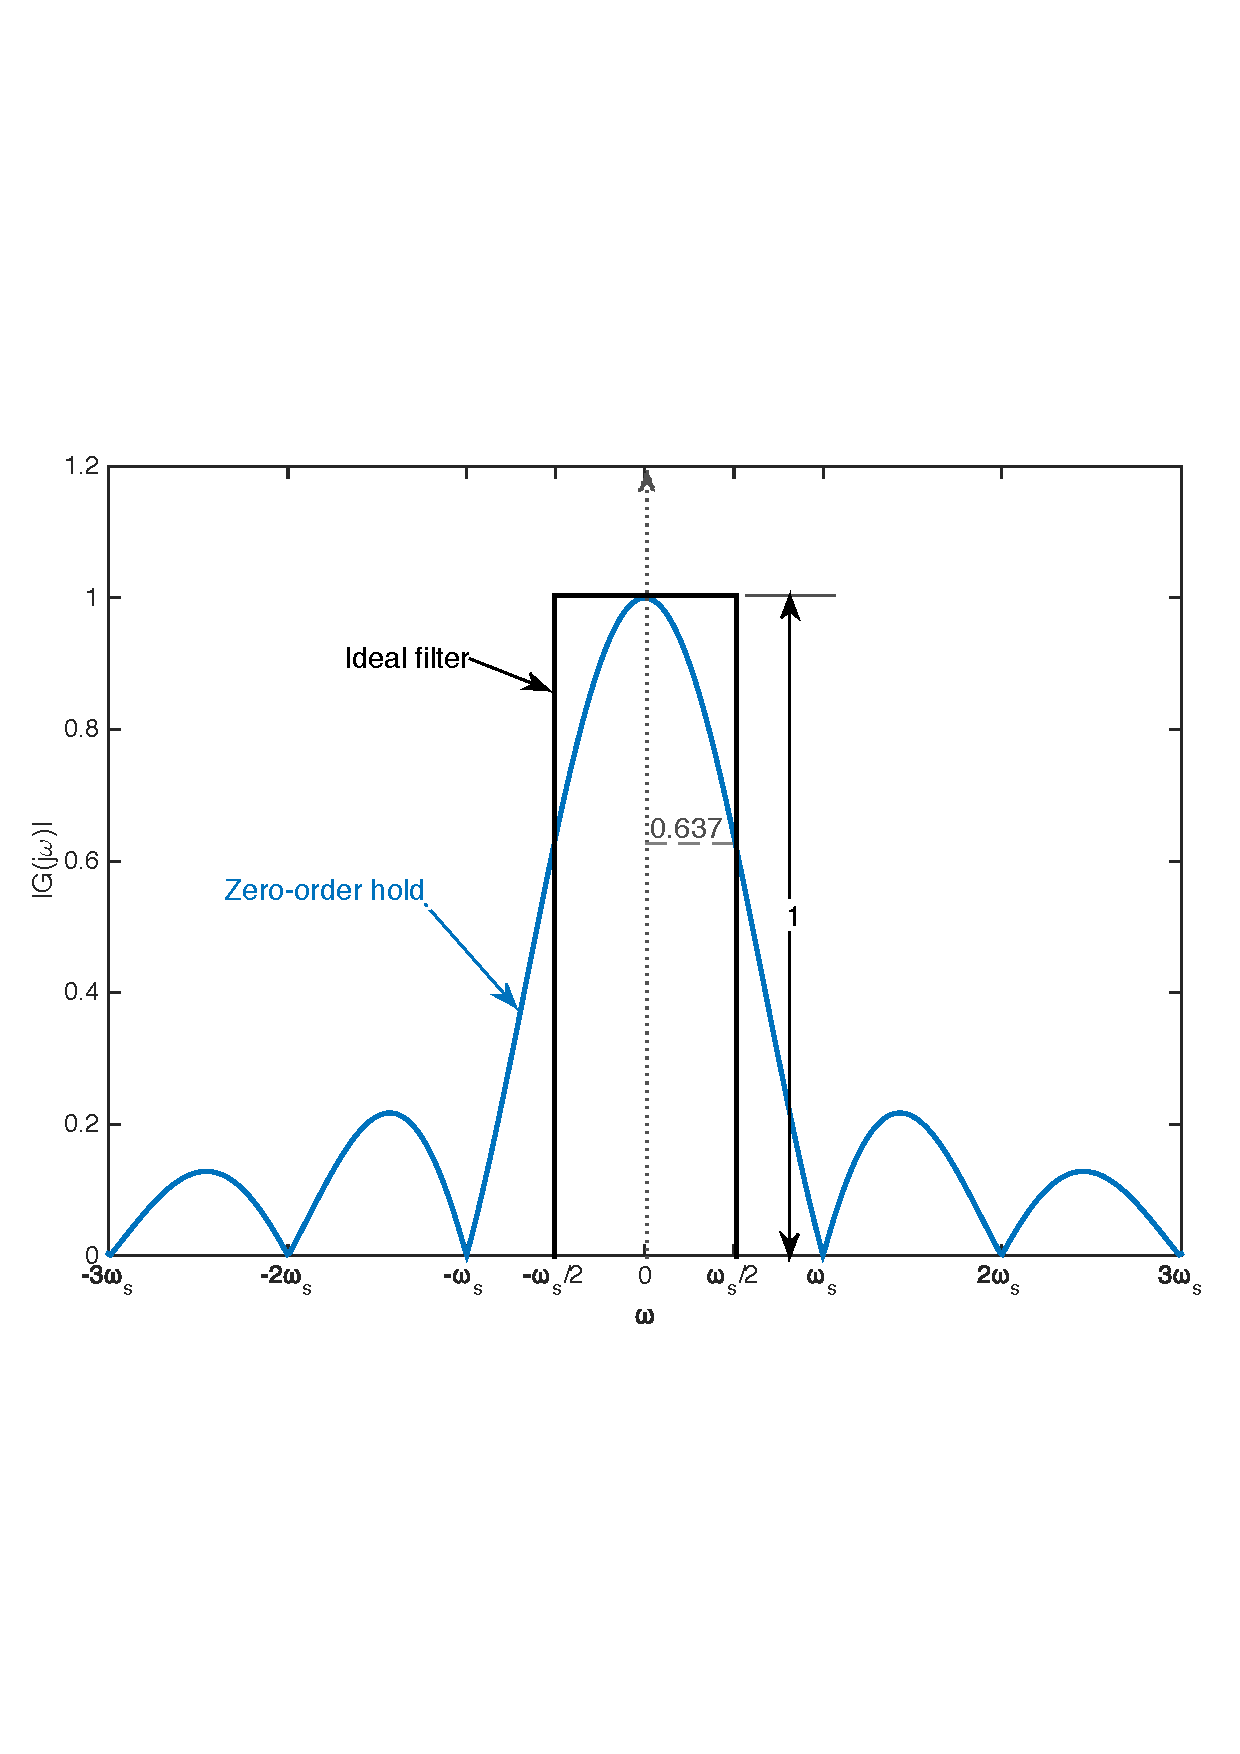
\includegraphics[width=0.8\linewidth]{zo_vs_ideal}
	\end{figure}
\end{frame}

\begin{frame}
	\frametitle{First-order hold}
	If the extrapolation is done by a first order polynomial, then the extrapolator is called a first-order hold and its transfer function is denoted $FOH(s)$. 
	\begin{center}
		$FOH(s)=(1-e^{-sT_s})\frac{sT_s+1}{sT_s^2}$
	\end{center}
	\vspace{-0.5em}
	\begin{figure}
		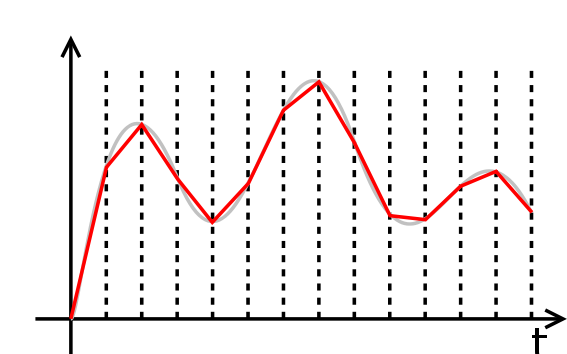
\includegraphics[width=0.5\linewidth]{foh}
	\end{figure}
\end{frame}

\section{Block-diagram analysis of sampled-data systems}

\subsection{General Approach}

\begin{frame}
	\frametitle{Problem Statement}
	\justify
	To analyse a feedback system that contains a digital controller, we need to be able to compute the transforms of output signals of systems that contain sampling operations in various places, including feedback loops, in the block diagram.\\
	\vspace{1em}
	The technique presented in this chapter is a simple extension of the block-diagram analysis of systems that are all continuous or all discrete. However a couple of rules need to be carefully observed. 
\end{frame}

\begin{frame}
	\frametitle{Block-diagram analysis}
	\justify
	We represent the process of sampling a continuous signal and holding it by impulse modulation followed by low-pass filtering. For example the following system: 
	\vspace{1em}
	\begin{figure}
		\centering
		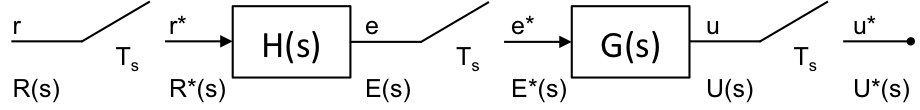
\includegraphics[width=1\linewidth]{block_analysis_1}
		\vspace{0.5em}
	\end{figure}
	leads to:
	\begin{equation}
		\begin{split}
		E(s) &= R^{*}(s)H(s)\\
		U(s) &= E^{*}(s)G(s)
		\end{split}
	\end{equation}
\end{frame}

\begin{frame}
	\frametitle{Block-diagram analysis}
	\begin{block}{Relation I}
		\justify
		If the transform of the signal to be sampled is a product of a transform that is already periodic of period $\frac{2\pi}{T_s}$, and one that is not, as in $U(s) = E^{*}(s)G(s)$, where $E^{*}(s)$ is periodic and $G(s)$ is not, we can show that $E^{*}(s)$ comes out as a factor, resulting in the following rule: 
		\begin{equation}
		U^{*}(s) = \big(E^{*}(s)G(s)\big)^{*} = E^{*}(s)G^{*}(s)
		\end{equation}
	\end{block}
	\vspace{1em}
	We will prove this in the frequency domain, using $R^*(s)=\frac{1}{T_s}\sum_{n=-\infty}^{\infty}R(s-jn\omega_s)$.\\
\end{frame}

\begin{frame}
	\frametitle{Proof of $U^{*}(s) = \big(E^{*}(s)G(s)\big)^{*} = E^{*}(s)G^{*}(s)$}
	If $U(s) = E^{*}(s)G(s)$, then by definition we have:
	\begin{equation}
	U^{*}(s) = \frac{1}{T_s} \sum_{n=-\infty}^{\infty} E^{*}(s - jn\omega_s)G(s - jn\omega_s),
	\end{equation}
	but $E^{*}(s)$ is
	\begin{equation}
	E^{*}(s) = \frac{1}{T_s} \sum_{k=-\infty}^{\infty} E(s-jk\omega_s),
	\end{equation}
	so that
	\begin{equation}
	E^{*}(s-jn\omega_s) = \frac{1}{T_s} \sum_{k=-\infty}^{\infty} E(s - jk\omega_s - jn\omega_s).
	\end{equation}
\end{frame}

\begin{frame}
	\frametitle{Proof of $U^{*}(s) = \big(E^{*}(s)G(s)\big)^{*} = E^{*}(s)G^{*}(s)$}
	Now in Eq.(6) we can let $k = l - n$ to get
	\begin{equation}
	\begin{split}
	E^{*}(s-jn\omega_s) &= \frac{1}{T_s} \sum_{l=-\infty}^{\infty} E(s - jl\omega_s)\\
	&= E^{*}(s)
	\end{split}
	\end{equation}
	\justify
	In other words, because $E^{*}$ is already periodic, shifting it an integral number of periods leaves it unchanged. Substituting Eq.(7) into Eq.(4) yiels
	\begin{equation}
	\begin{split}
	U^{*}(s) &= E^{*}(s) \frac{1}{T_s} \sum_{-\infty}^{\infty} G(s - jn\omega_s)\\
	&= E^{*}(s)G^{*}(s)
	\end{split}
	\end{equation}
\end{frame}

\begin{frame}
	\frametitle{Block diagram analysis}
	\begin{alertblock}{Note what is not true}
		\justify
		If $U(s) = E(s)G(s)$, then $U^{*}(s) \neq E^{*}(s) G^{*}(s)$ but rather $U^{*}(s) = (EG)^{*}(s)$. The periodic character of $E^{*}$ in Eq.(3) is crucial.
	\end{alertblock}
	\vspace{1em}
	\begin{block}{Relation II}
		\justify
		Given a sampled-signal transform such as $U^{*}(s)$, we can find the corresponding $\mathcal{Z}$-transform simply by letting $e^{sT_s} = z$ or $U(z) = U^{*}(s)|_{e^{sT_s} = z}$.
	\end{block}
\end{frame}

\subsection{Examples}

\begin{frame}
	\begin{exampleblock}{Example 1 (1/4)}
		Let's compute the discrete-time representation of the following block diagram:
		\vspace{-1em}
		\begin{figure}
		\centering
		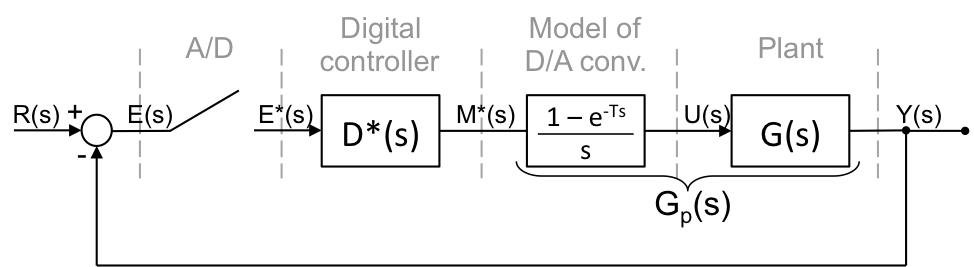
\includegraphics[width=1\linewidth]{block_analysis_2}
		\end{figure}
		From the diagram we have that:
		\vspace{-1em} 
		\begin{equation}
			E(s) = R(s) - Y(s)
			\vspace{-1em}
		\end{equation}
		\begin{equation}
			Y(s) = G_p(s)D^{*}(s)E^{*}(s)
		\end{equation}
	\end{exampleblock}
\end{frame}

\begin{frame}
	\begin{exampleblock}{Example 1 (2/4)}
		Applying Relation I on both Eq.(9) and Eq.(10) results in:
		\begin{equation}
		E^{*}(s) = R^{*}(s) - Y^{*}(s)
		\end{equation}
		\begin{equation}
		Y^{*}(s) = \big ( G_p(s)D^{*}(s)E^{*}(s) \big )^{*} = G_p^{*}(s)D^{*}(s)E^{*}(s)
		\vspace{1.5em}
		\end{equation}
		Next we insert Eq.(11) in Eq.(12):
		\begin{equation}
		Y^{*}(s) = G_p^{*}(s)D^{*}(s) \big ( R^{*}(s) - Y^{*}(s) \big)
		\end{equation}
	\end{exampleblock}
\end{frame}

\begin{frame}
	\begin{exampleblock}{Example 1 (3/4)}
		Finally we convert Eq.(13) into a transfer function:
		\begin{align*}
		Y^{*}(s) &= G_p^{*}(s)D^{*}(s) \big ( R^{*}(s) - Y^{*}(s) \big)\\
		Y^{*}(s) + G_p^{*}(s)D^{*}(s)Y^{*}(s) &= G_p^{*}(s)D^{*}(s)R^{*}(s)\\
		Y^{*}(s) \big (1 +  G_p^{*}(s)D^{*}(s) \big) &= G_p^{*}(s)D^{*}(s)R^{*}(s)\\
		\frac{Y^{*}(s)}{R^{*}(s)} &= \frac{G_p^{*}(s)D^{*}(s)}{1 +  G_p^{*}(s)D^{*}(s)}\\
		\frac{Y(z)}{R(z)} &= \frac{G_p(z)D(z)}{1 +  G_p^(z)D(z)}
		\end{align*}
		The last expression is obtained by applying Relation II.
	\end{exampleblock}
\end{frame}

\begin{frame}
	\begin{exampleblock}{Example 1 (4/4)}
		\justify		
		Notice that the resulting transfer function is also the transfer function of the following discrete-time system:
		\begin{figure}
			\centering
			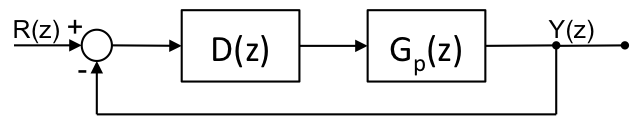
\includegraphics[width=0.8\linewidth]{block_analysis_3}
		\end{figure}
		Consequently, we have found a discrete-time equivalent of a system which contains continuous-time and sampled signals.
	\end{exampleblock}
\end{frame}

\begin{frame}
	\begin{exampleblock}{Example 2 (1/3)}
		Let's compute the discrete-time representation of the following block diagram:
		\vspace{-1.5em}
		\begin{figure}
			\centering
			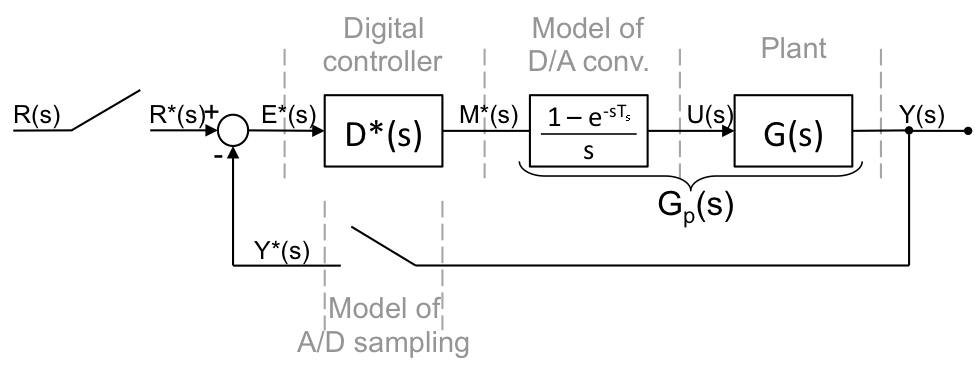
\includegraphics[width=1\linewidth]{block_analysis_4}
			\vspace{-1.5em}
		\end{figure}
		From the diagram we have that: 
		\vspace{-1em}
		\begin{equation}
		E^{*}(s) = R^{*}(s) - Y^{*}(s)
		\vspace{-1em}
		\end{equation}
		\begin{equation}
		Y(s) = G_p(s)D^{*}(s)E^{*}(s)
		\end{equation}
	\end{exampleblock}
\end{frame}

\begin{frame}
	\begin{exampleblock}{Example 2 (2/3)}
		Applying Relation I on Eq.(15), yields:
		\begin{equation}
		Y^{*}(s) = \big ( G_p(s)D^{*}(s)E^{*}(s) \big )^{*} = G_p^{*}(s)D^{*}(s)E^{*}(s)
		\end{equation}
		Next we insert Eq.(14) in Eq.(16):
		\begin{equation}
		Y^{*}(s) = G_p^{*}(s)D^{*}(s) \big ( R^{*}(s) - Y^{*}(s) \big)
		\end{equation}
		This is the exact same expression as we have for example 1. We will find the same transfer function from Eq.(17).
	\end{exampleblock}
\end{frame}

\begin{frame}
	\begin{exampleblock}{Example 2 (3/3)}
		\justify		
		The transfer function:
		\begin{center}
			$\frac{Y(z)}{R(z)} = \frac{G_p(z)D(z)}{1 +  G_p^(z)D(z)}$
		\end{center}
		is also the transfer function of the following discrete-time system:
		\begin{figure}
			\centering
			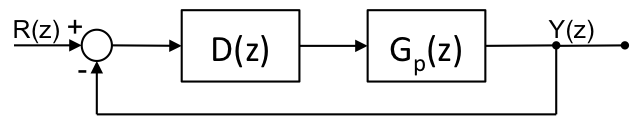
\includegraphics[width=0.8\linewidth]{block_analysis_3}
		\end{figure}
		Consequently, we have found a discrete-time equivalent of a system which contains continuous-time and sampled signals.
	\end{exampleblock}
\end{frame}

\begin{frame}
	\begin{alertblock}{NOTE}
	\begin{center}
		$G_p^{*}(s) = \big[ \frac{(1 - e^{-sT_s})}{s} G(s) \big]^{*}$
	\end{center}
	Taking out the periodic parts, which are those in which s appears only as $e^{sT_s}$, we have that
	\begin{center}
		$G_p^{*}(s) = (1 - e^{-sT_s}) \big[ \frac{G(s)}{s} \big]^{*}$
	\end{center}
	Letting $e^{sT_s} = z$, we have that:
	\begin{center}
		$G_p(z) = (1-z^{-1}) \mathcal{Z} \big\{ \frac{G(s)}{s} \big\}$
	\end{center}
	\end{alertblock}
\end{frame}